\documentclass{article}

\usepackage{Sweave}
\begin{document}
\Sconcordance{concordance:seguimientov3.tex:seguimientov3.Rnw:%
1 2 1 1 0 16 1 1 5 1 29 15 0 1 3 4 1 1 7 1 2 4 1 1 7 1 3 4 1 1 7 1 3 4 %
1 1 7 1 3 4 1 1 7 1 3 4 1 1 5 1 3 4 1 1 6 1 3 4 1 1 6 1 3 4 1 1 6 1 3 4 %
1 1 6 1 3 4 1 1 6 1 3 4 1 1 6 1 3 4 1 1 6 1 3 4 1 1 6 1 3 4 1 1 6 1 3 4 %
1 1 6 1 3 4 1 1 6 1 3 4 1 1 6 1 3 4 1 1 6 1 3 4 1 1 6 1 3 4 1 1 6 1 3 4 %
1 1 6 1 3 4 1 1 6 1 3 4 1 1 6 1 3 4 1 1 6 1 3 4 1 1 6 1 3 4 1 1 6 1 3 4 %
1 1 6 1 3 4 1 1 6 1 3 5 1 6 0 1 5 1 1 1 6 15 0 1 3 3 1 1 7 1 2 4 1 1 7 %
1 3 4 1 1 7 1 3 4 1 1 7 1 3 4 1 1 7 1 3 4 1 1 5 1 3 4 1 1 6 1 3 4 1 1 6 %
1 3 4 1 1 6 1 3 4 1 1 6 1 3 4 1 1 6 1 3 4 1 1 6 1 3 4 1 1 6 1 3 4 1 1 6 %
1 3 4 1 1 6 1 3 4 1 1 6 1 3 4 1 1 6 1 3 4 1 1 6 1 3 4 1 1 6 1 3 4 1 1 6 %
1 3 4 1 1 6 1 3 4 1 1 6 1 3 4 1 1 6 1 3 4 1 1 6 1 3 4 1 1 6 1 3 4 1 1 6 %
1 3 4 1 1 6 1 3 4 1 1 6 1 3 4 1 1 6 1 3 5 1 6 0 1 5 1 1 1 6 15 0 1 3 3 %
1 1 7 1 2 4 1 1 7 1 3 4 1 1 7 1 3 4 1 1 7 1 3 4 1 1 7 1 3 4 1 1 5 1 3 4 %
1 1 6 1 3 4 1 1 6 1 3 4 1 1 6 1 3 4 1 1 6 1 3 4 1 1 6 1 3 4 1 1 6 1 3 4 %
1 1 6 1 3 4 1 1 6 1 3 4 1 1 6 1 3 4 1 1 6 1 3 4 1 1 6 1 3 4 1 1 6 1 3 4 %
1 1 6 1 3 4 1 1 6 1 3 4 1 1 6 1 3 4 1 1 6 1 3 4 1 1 6 1 3 4 1 1 6 1 3 4 %
1 1 6 1 3 4 1 1 6 1 3 4 1 1 6 1 3 4 1 1 6 1 3 4 1 1 6 1 3 3 1}

\title{PROMSACE: Seguimiento de encuestas}
\author{Hernan Nuñez}
\date{\today}
\maketitle
\begin{abstract}
Lo mostrado en este documento nos da una vision descriptiva y exploratoria sobre los cambios a traves del tiempo (del 28 febrero al 30 de junio) de las encuestas recopiladas y completas. Se trabajo con Latex y RStudio. Pueden encontrar el codigo en https://github.com/HernanPerci/PROMSACE
\end{abstract}

\tableofcontents

\section{Introduccion}
La encuesta sobre la que se respalda el presente informe aun se esta recolectando mediante la platafoma surveymonkey.

\section{Variables de estudio}


\begin{Schunk}
\begin{Soutput}
Rows: 2,235
Columns: 10
$ Fecha                            <dttm> 2020-06-30, 2020-06-29, 2020-06-2...
$ Hora                             <dbl> 21, 21, 14, 14, 12, 21, 21, 17, 12...
$ Dia                              <dbl> 30, 29, 29, 29, 29, 28, 26, 26, 26...
$ `Dia de la semana`               <fct> martes, lunes, lunes, lunes, lunes...
$ Mes                              <fct> Junio, Junio, Junio, Junio, Junio,...
$ `Organo de pertenencia`          <fct> asesoria, Sin respuesta, Sin respu...
$ Sexo                             <chr> "Hombre", "Sin respuesta", "Sin re...
$ `Tiempo trabajando en el Estado` <fct> <10 a mas>, Sin respuesta, Sin res...
$ `Nivel de gobierno`              <fct> Regional, Sin respuesta, Sin respu...
$ `Encuesta completa`              <chr> "Si", "No", "No", "Si", "No", "Si"...
\end{Soutput}
\end{Schunk}

\section{Panorama general del 28 de Febrero al 30 de Junio}

\subsection{Cantidad de encuestas completas e incompletas por fecha y Hora}

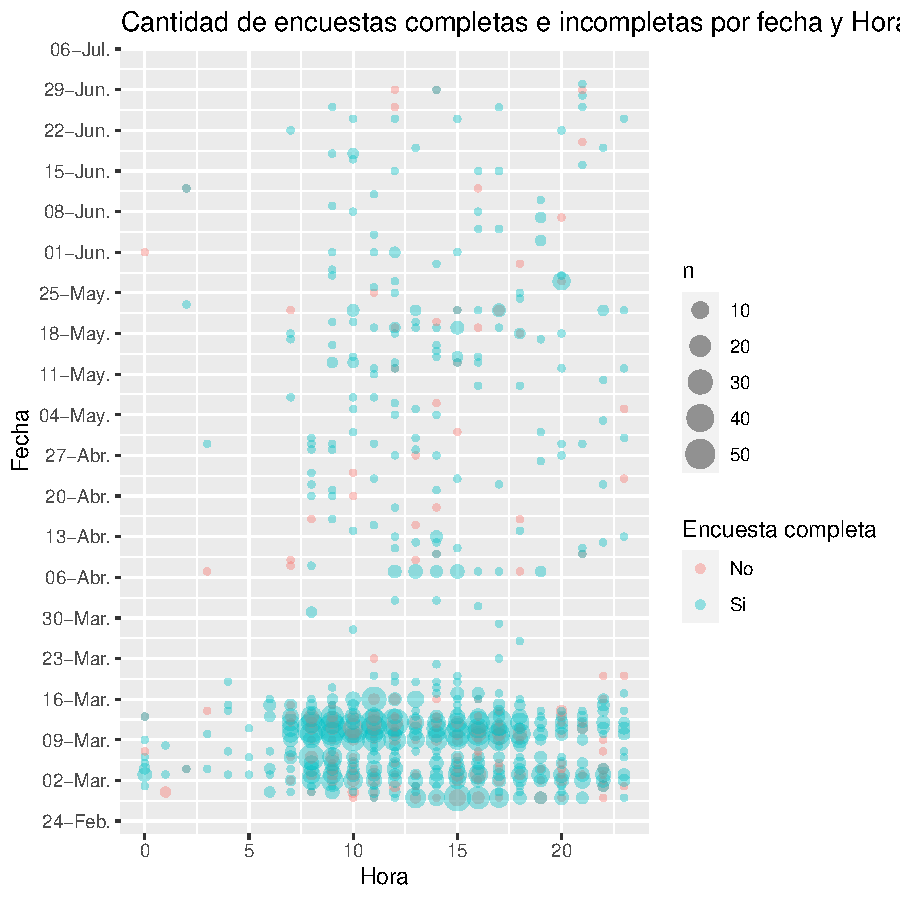
\includegraphics{seguimientov3-003}

Se puede apreciar que hubo mayor recepcion de encuestas diarias hasta el lunes 16 de Marzo y en horario de trabajo.

\subsection{Cantidad de encuestas completas e incompletas por fecha y organo de pertenencia}

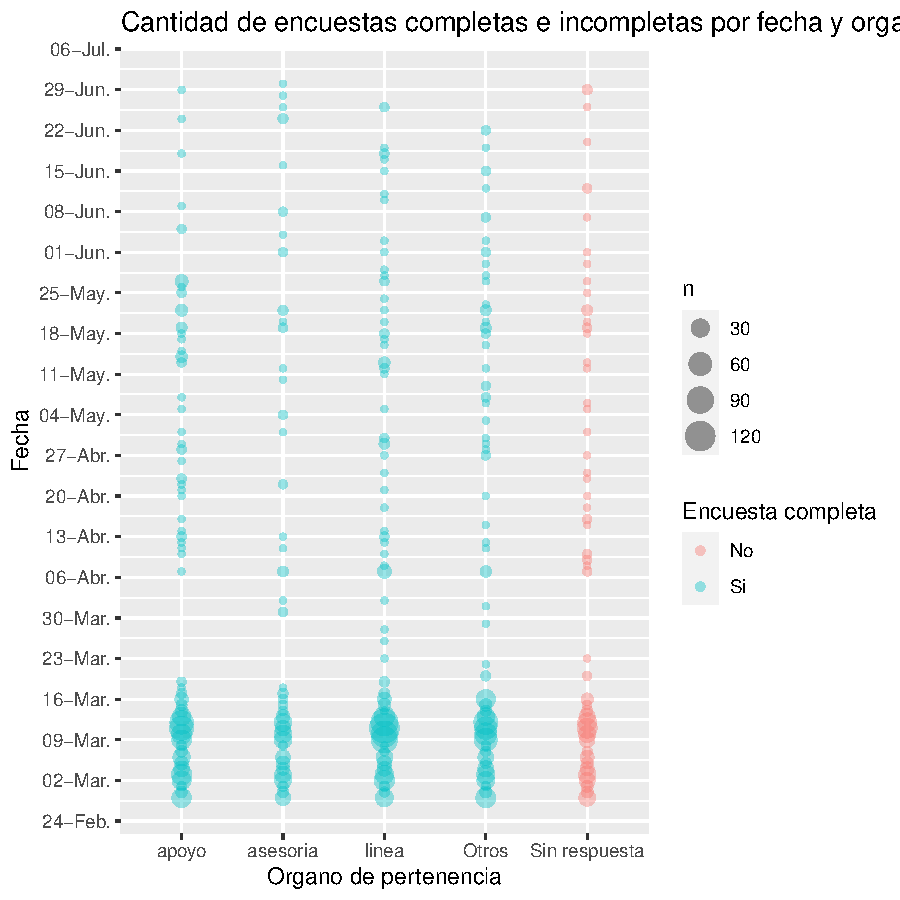
\includegraphics{seguimientov3-004}

Vemos graficamente que los de organo de linea fueron los que mas contestaban antes del 16 de Marzo.

\subsection{Cantidad de encuestas completas e incompletas por fecha y sexo}

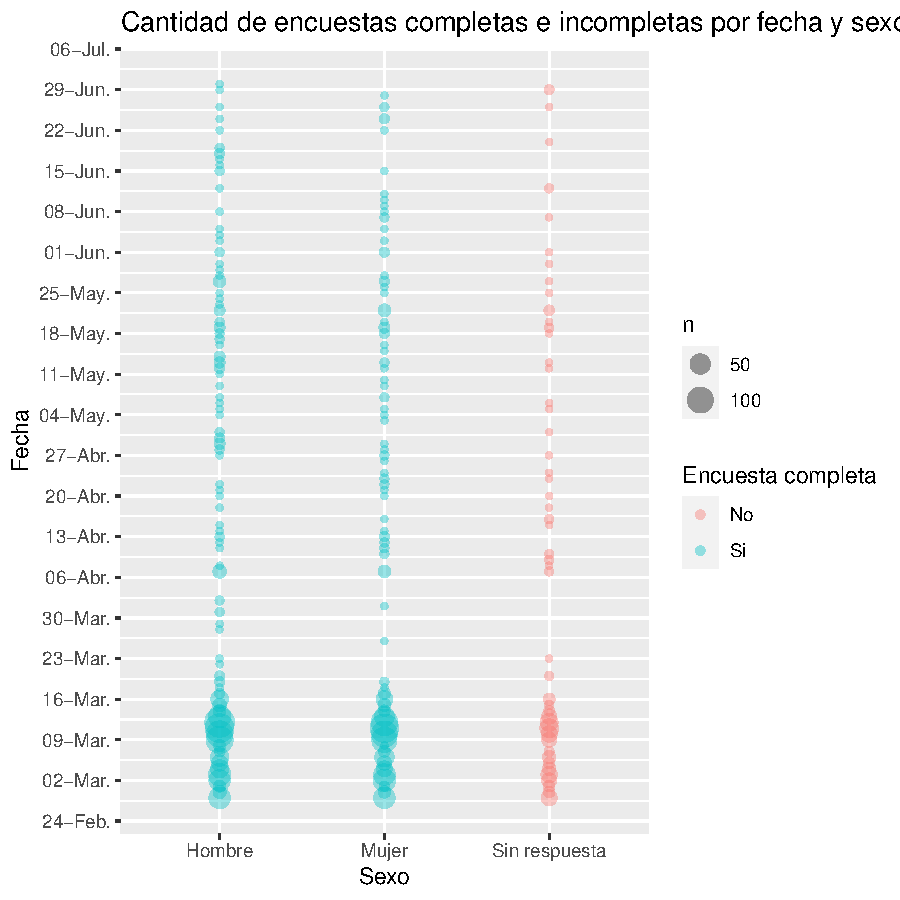
\includegraphics{seguimientov3-005}

La proporcion de respuestas entre hombre y mujeres se ve similar en todo el periodo desde el 28 de febrero hasta el 30 de junio, con la aclaracion que se redujeron similarmente las respuestas a partir del 16.

\subsection{Cantidad de encuestas completas e incompletas por fecha y tiempo trabajando en el estado}

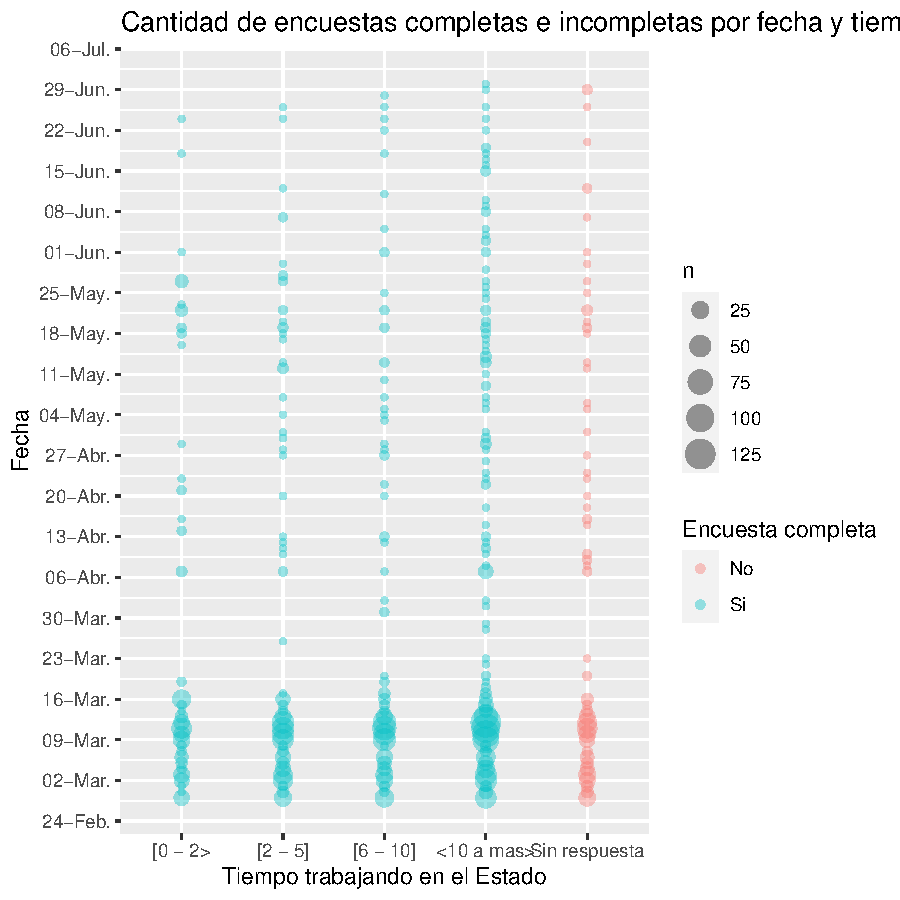
\includegraphics{seguimientov3-006}

Antes del 16 de Marzo habian respondido en mayor numero a las encuestas los que estan trabajan de 10 años a mas.

\subsection{Cantidad de encuestas completas e incompletas por fecha y nivel de gobierno}

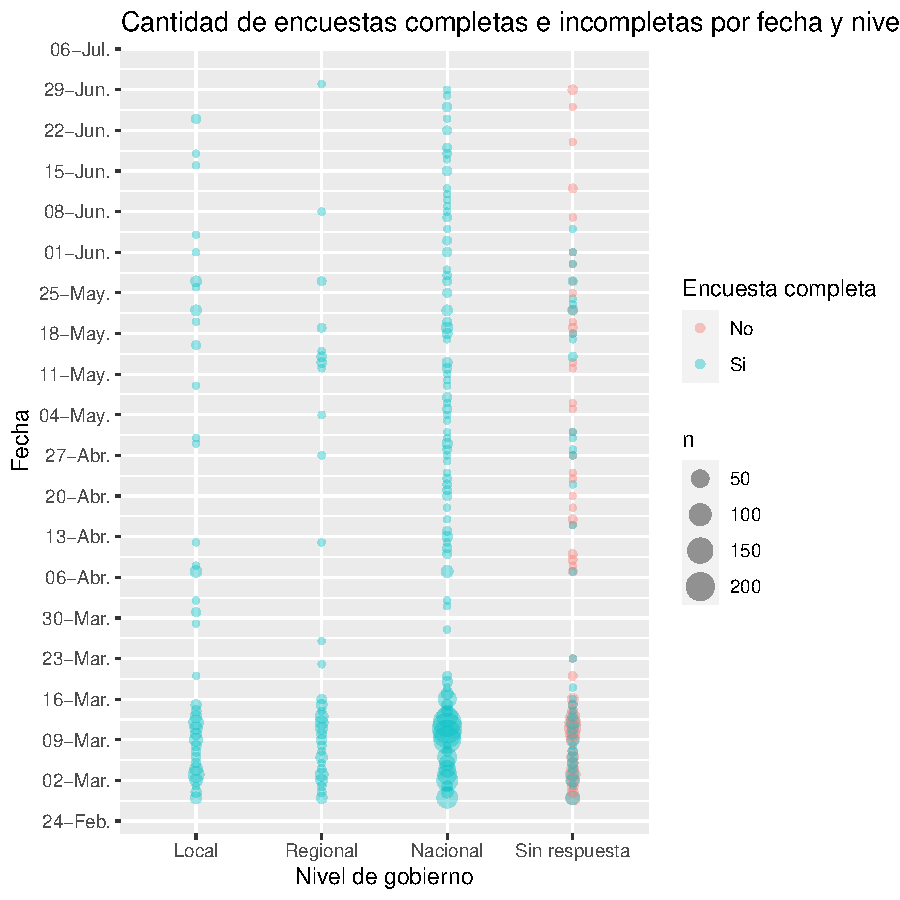
\includegraphics{seguimientov3-007}

Antes del 16 de Marzo obtuvimos mayores cantidades de respuestas del nivel de gobierno Nacional.

\subsection{Cantidad de encuestas completas e incompletas por hora y dia}

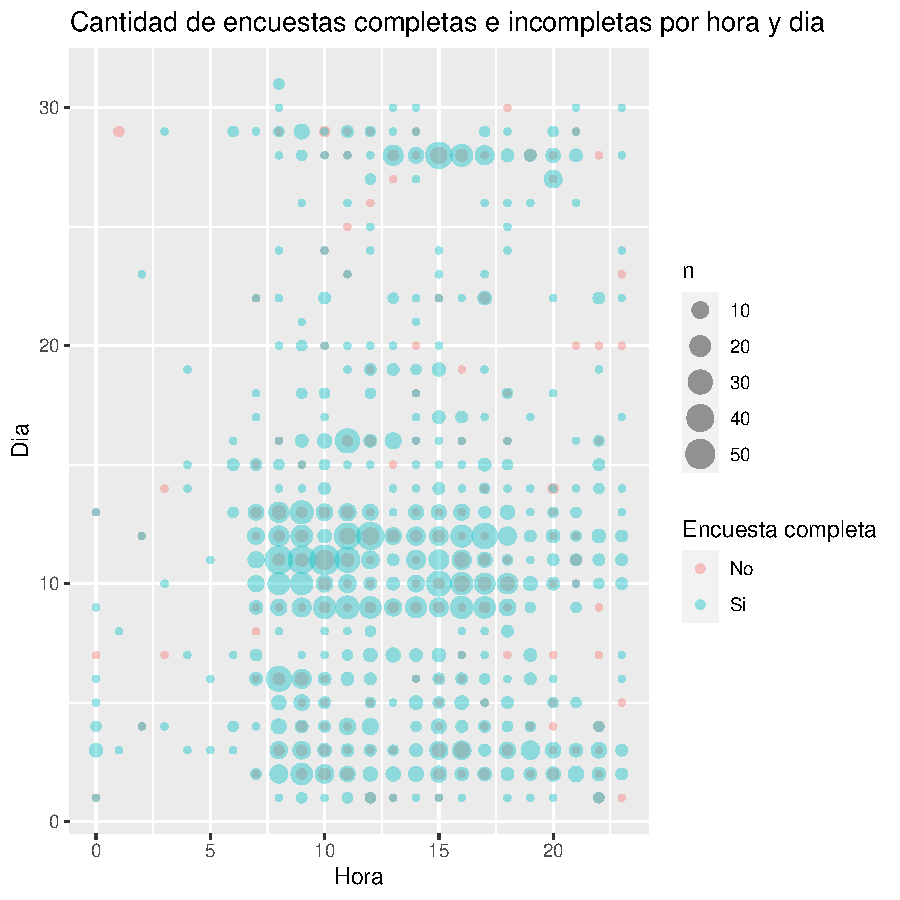
\includegraphics{seguimientov3-008}

Se podria decir que respondian las encuestas generalmene en el horario de trabajo y antes de la quincena de mes.

\subsection{Cantidad de encuestas completas e incompletas por hora y dia de la semana}

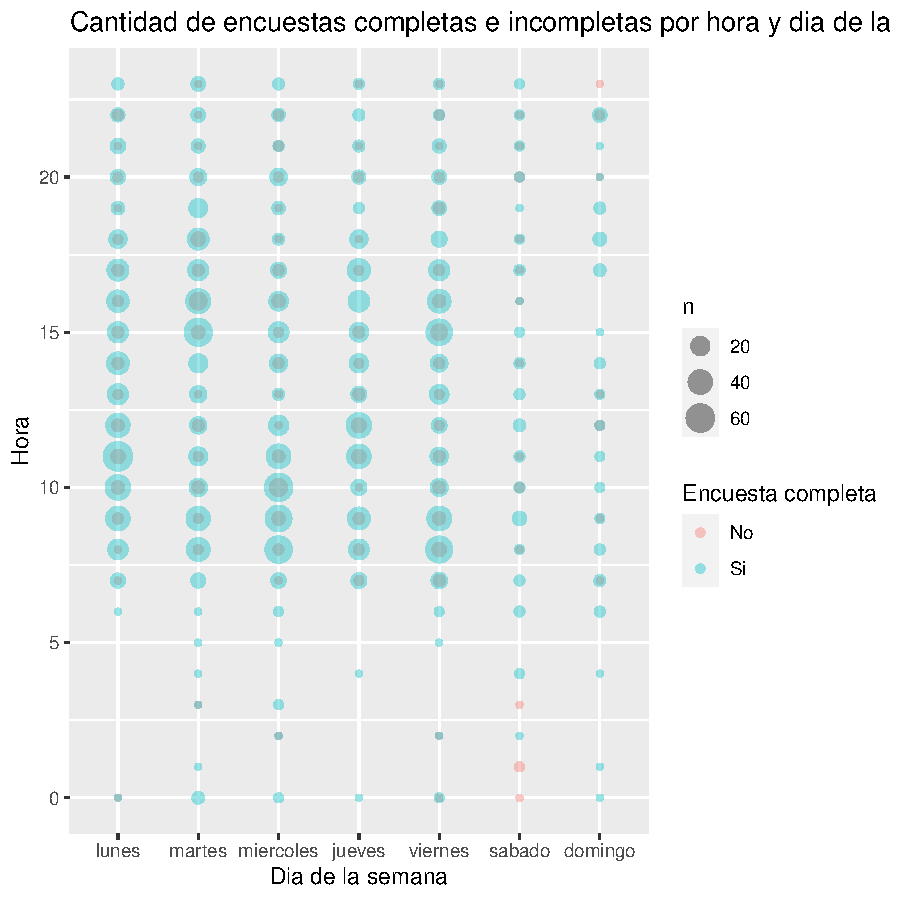
\includegraphics{seguimientov3-009}

En este grafico se aprecia mejor que mayormente respondieron a las encuestas en las horas de trabajo y en dias laborales de lunes a viernes.

\subsection{Cantidad de encuestas completas e incompletas por hora y mes}

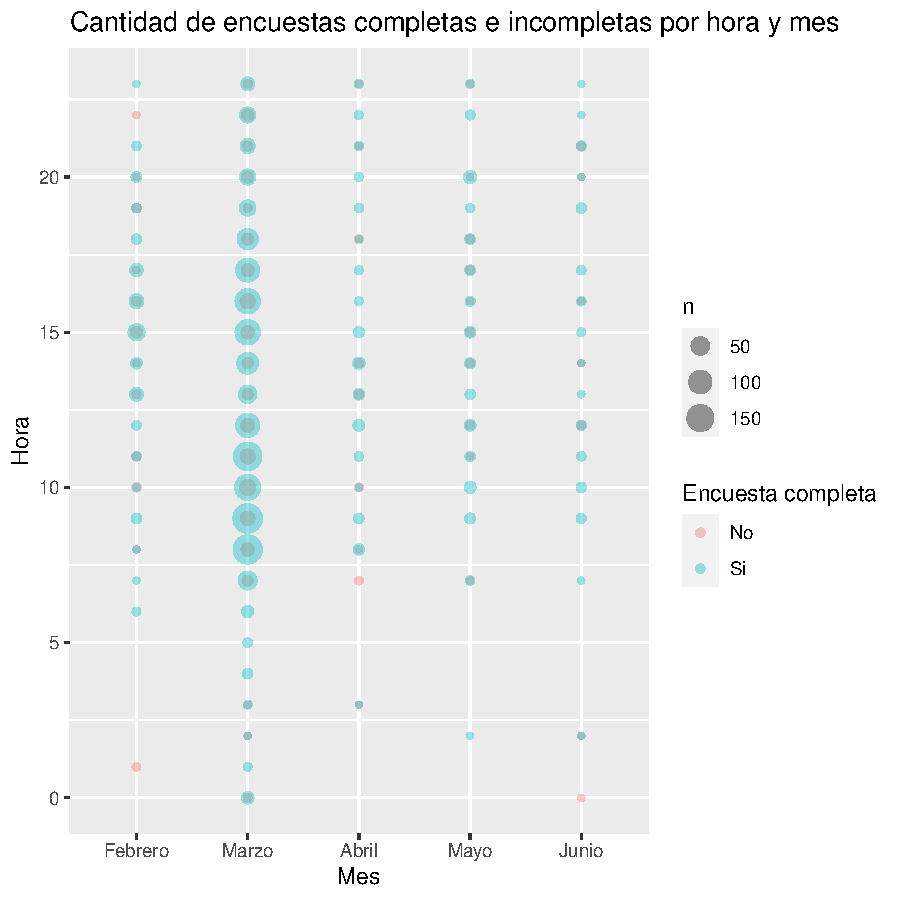
\includegraphics{seguimientov3-010}

En marzo es donde se obtubo mayor cantidad de respuestas en horarios laborales.

\subsection{Cantidad de encuestas completas e incompletas por hora y organo de pertenencia}

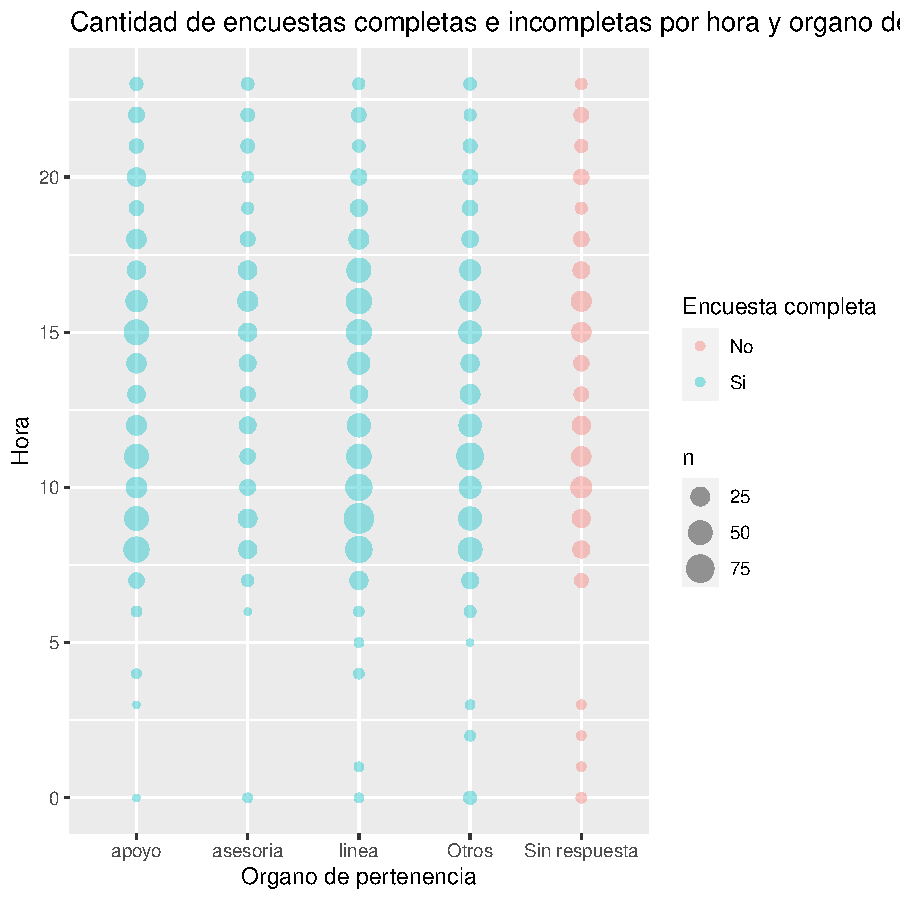
\includegraphics{seguimientov3-011}

A lo largo de las horas laborales los de organo de linea respondieron un poco mas con respecto a los demas.

\subsection{Cantidad de encuestas completas e incompletas por hora y sexo}

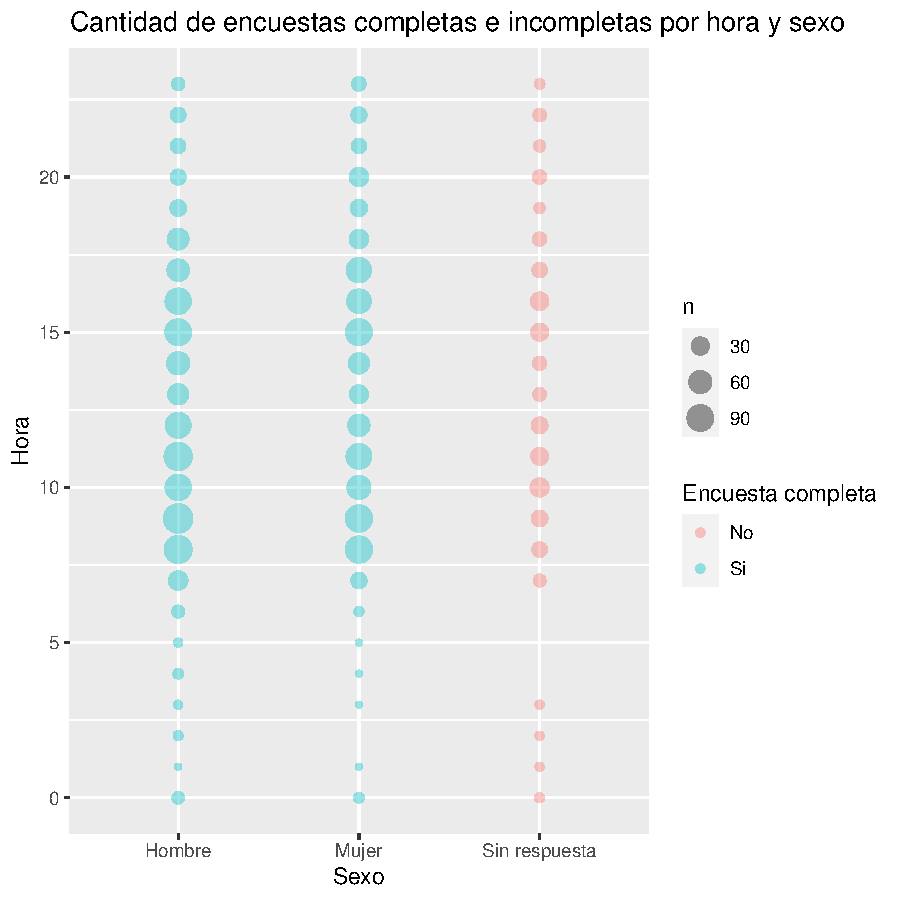
\includegraphics{seguimientov3-012}

Los hombres y las mujeres contestaron en similar proporcion durante las horas laborales.

\subsection{Cantidad de encuestas completas e incompletas por hora y tiempo trabajando en el estado}

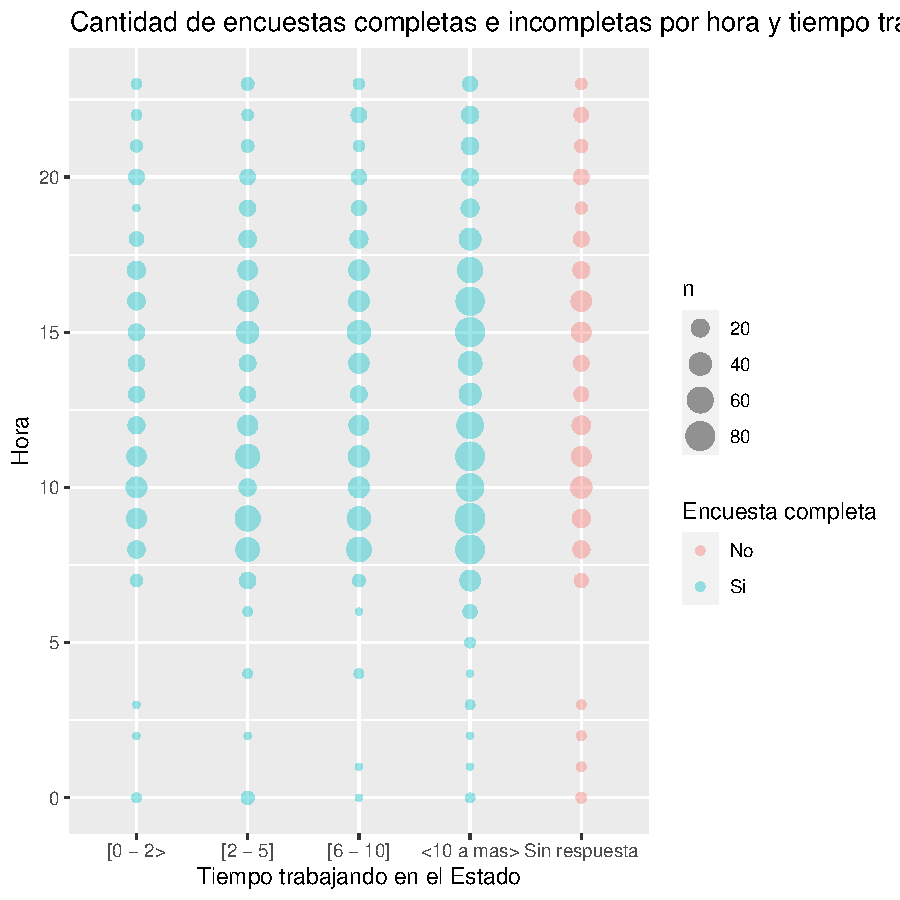
\includegraphics{seguimientov3-013}

Los que mas respondieron fueron los que trabajaron de 10 años a mas y durante el horario laboral.

\subsection{Cantidad de encuestas completas e incompletas por hora y nivel de gobierno}

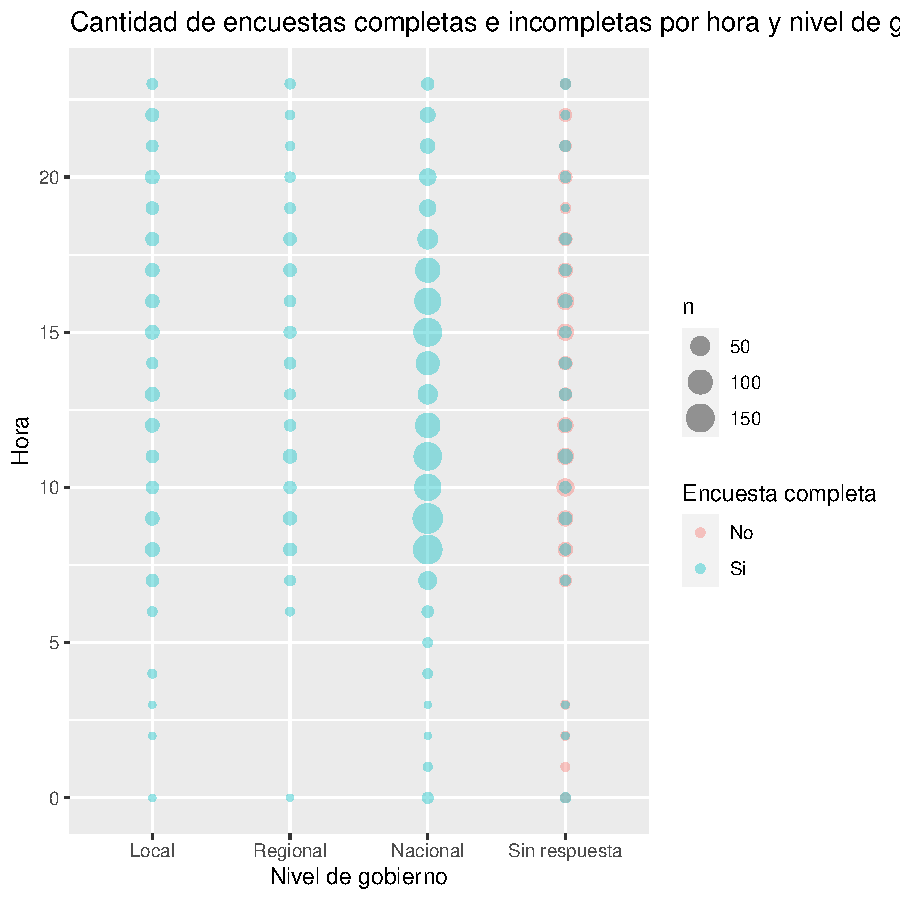
\includegraphics{seguimientov3-014}

Los de nivel de gobierno nacional fueron los que respondieron en mayor cantidad y en horario laboral.

\subsection{Cantidad de encuestas completas e incompletas por dia y mes}

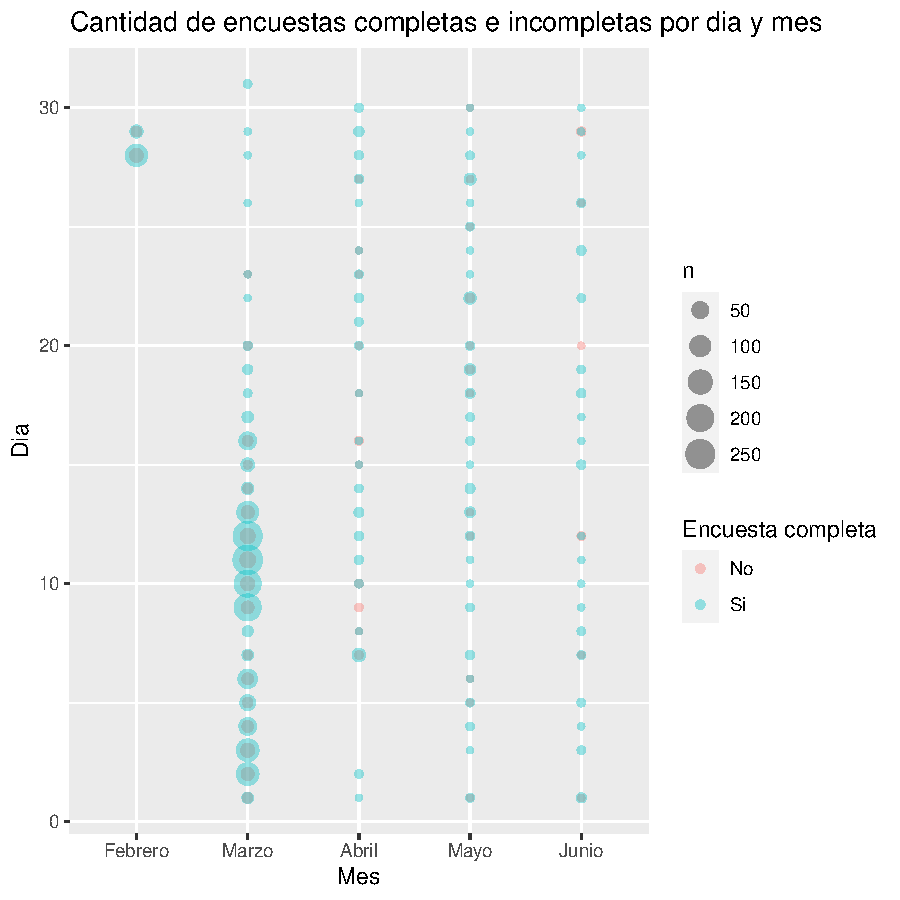
\includegraphics{seguimientov3-015}

Antes del 16 de Marzo se recopilaron la gran mayoria de encuestas que tenemos hasta el 30 de Junio.

\subsection{Cantidad de encuestas completas e incompletas por dia y organo de pertenencia}

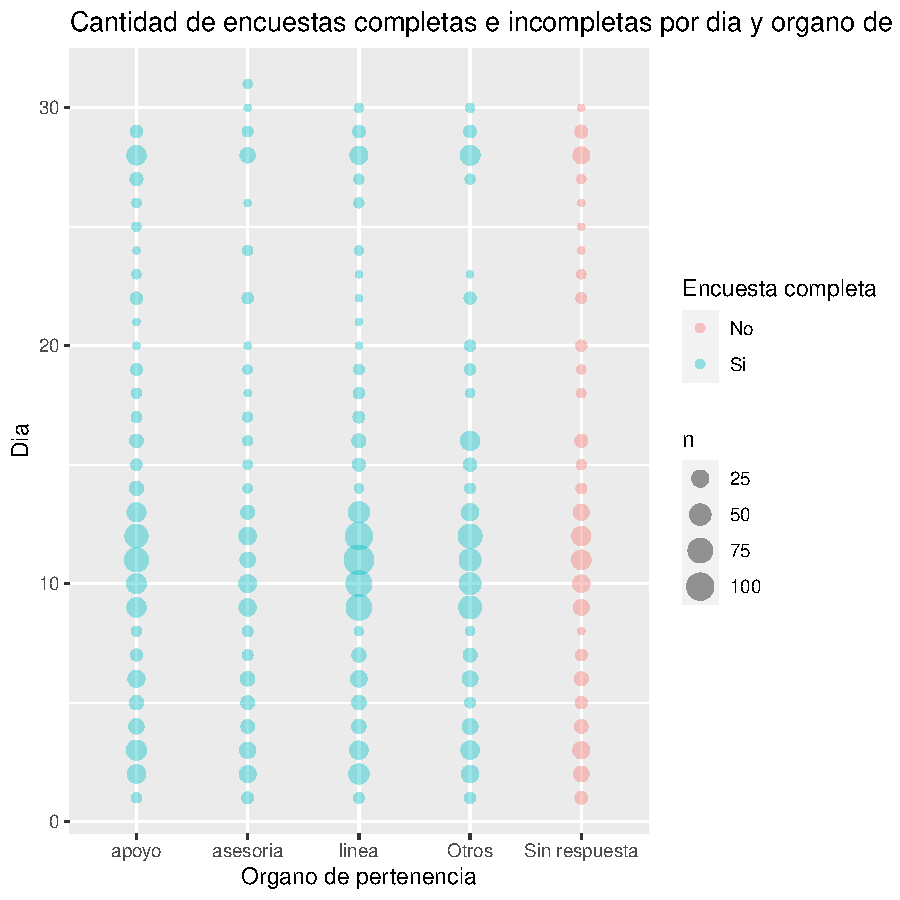
\includegraphics{seguimientov3-016}

Los de organo de linea fueron los que mas contestaron y lo hicieron generalmente alrededor del dia 10.

\subsection{Cantidad de encuestas completas e incompletas por dia y sexo}

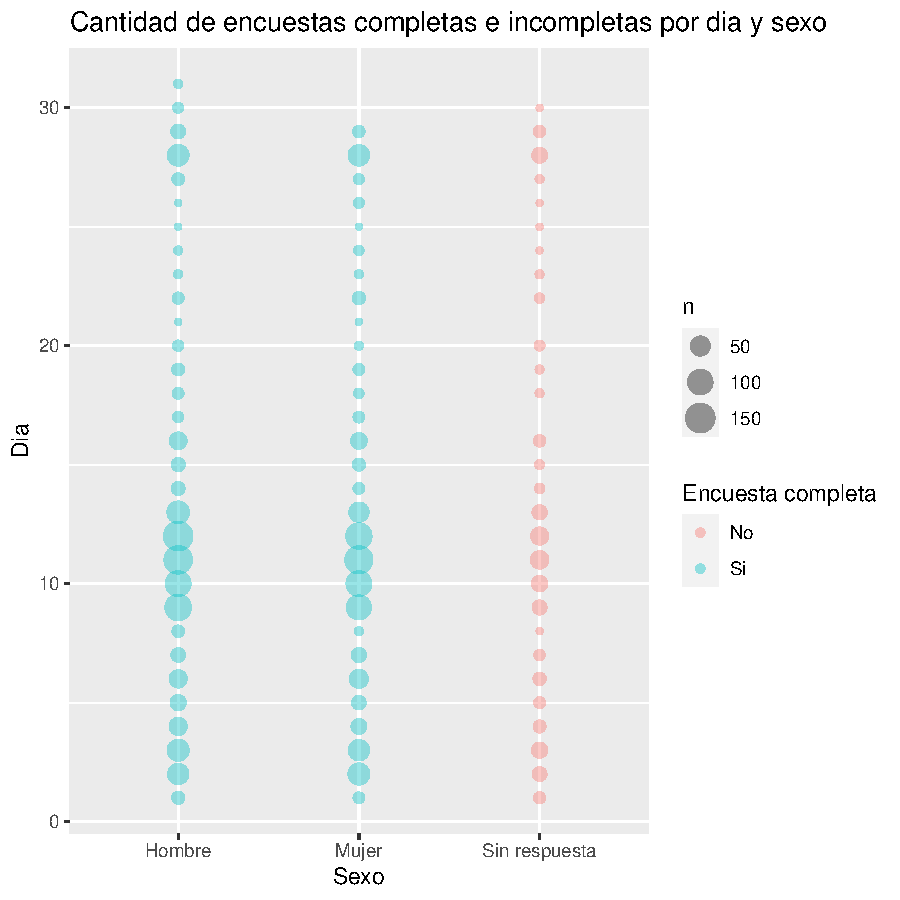
\includegraphics{seguimientov3-017}

La cantidad de encuestas recopiladas por hombres y mujeres fueron similares y de mayor cantidad alrededor del dia 10.

\subsection{Cantidad de encuestas completas e incompletas por dia y tiempo trabajando en el estado}

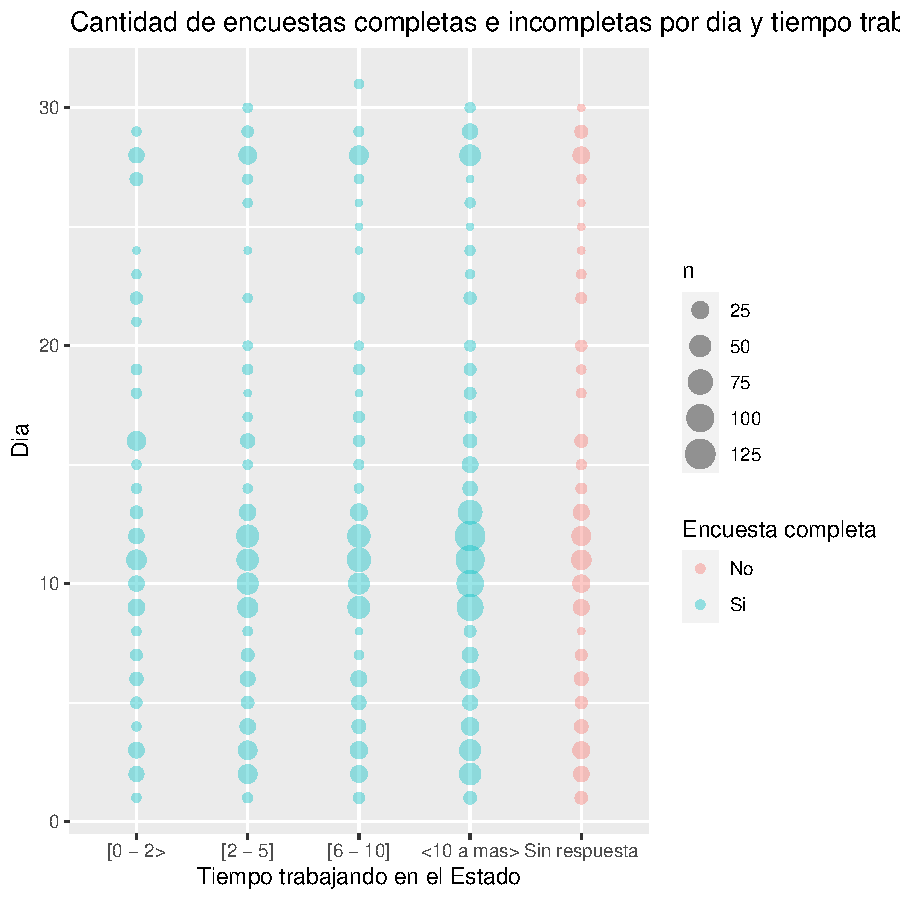
\includegraphics{seguimientov3-018}

Los que tienen de 10 a mas años trabajando en el estado fueron los que mas respondieron y alrededor del dia 10.

\subsection{Cantidad de encuestas completas e incompletas por dia y nivel de gobierno}

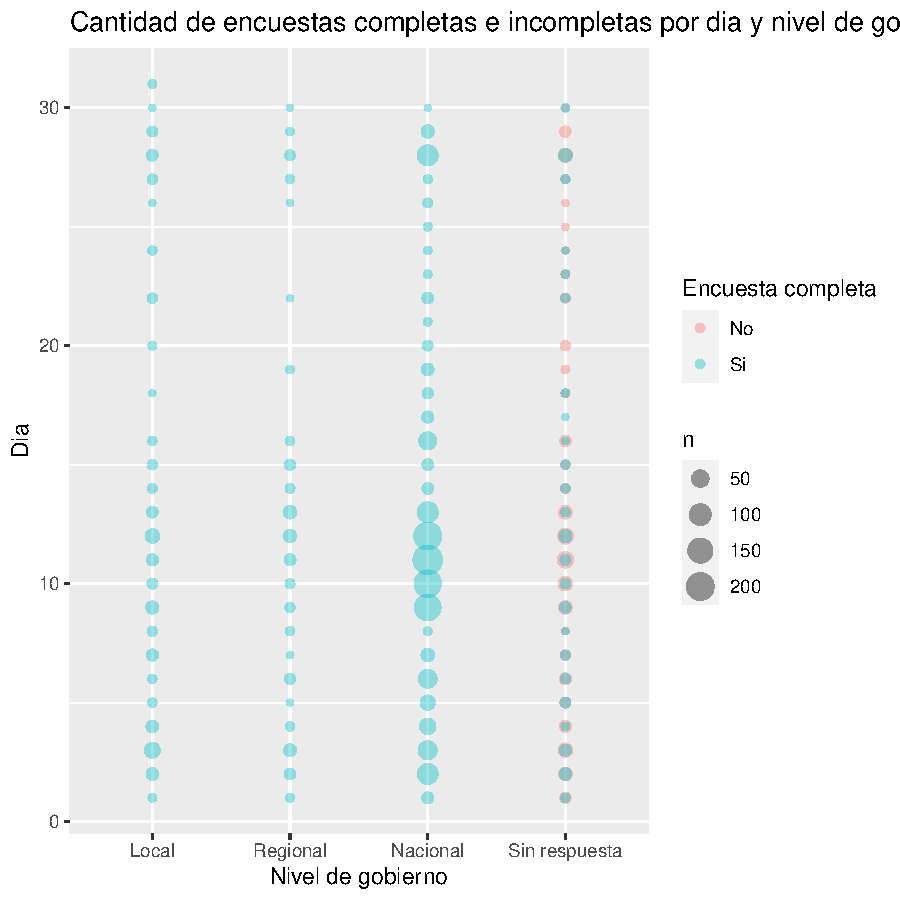
\includegraphics{seguimientov3-019}

Hubo mayor recepcion de respuestas departe del nivel de gobierno nacional y lo hicieron mayormente alrededor del dia 10.

\subsection{Cantidad de encuestas completas e incompletas por dia de la semana y mes}

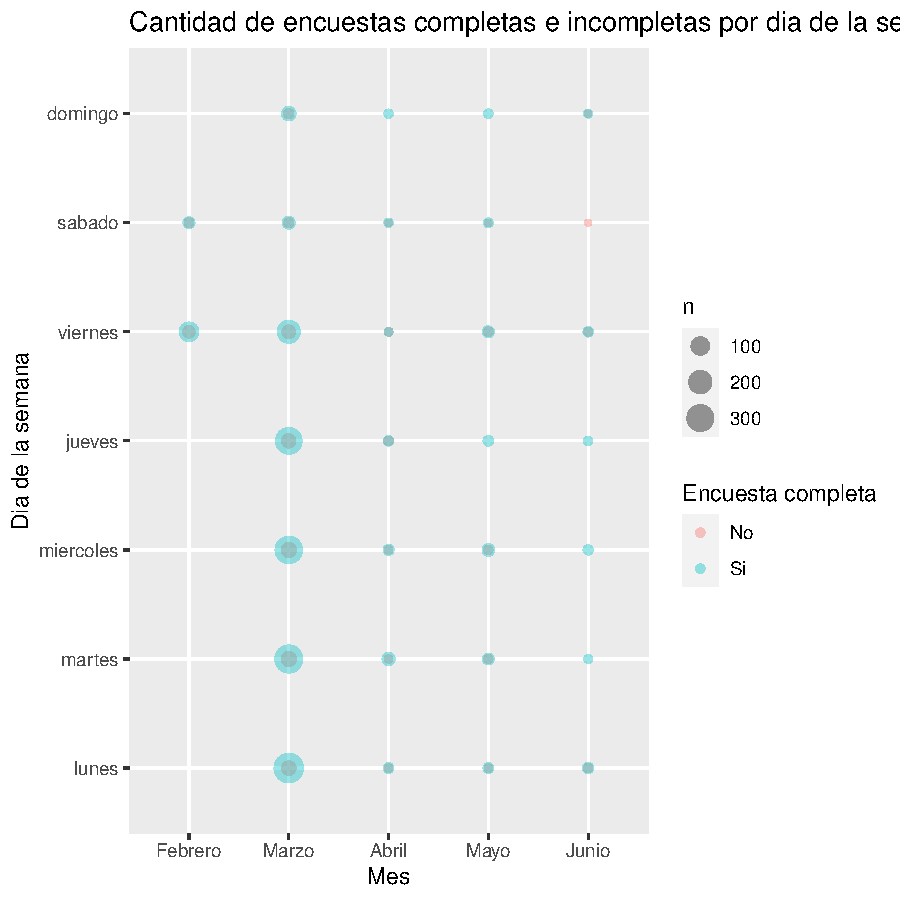
\includegraphics{seguimientov3-020}

Fue en Marzo y de lunes a viernes donde se obtuvo la mayor cantidad de respuestas.

\subsection{Cantidad de encuestas completas e incompletas por dia de la semana y organo de pertenencia}

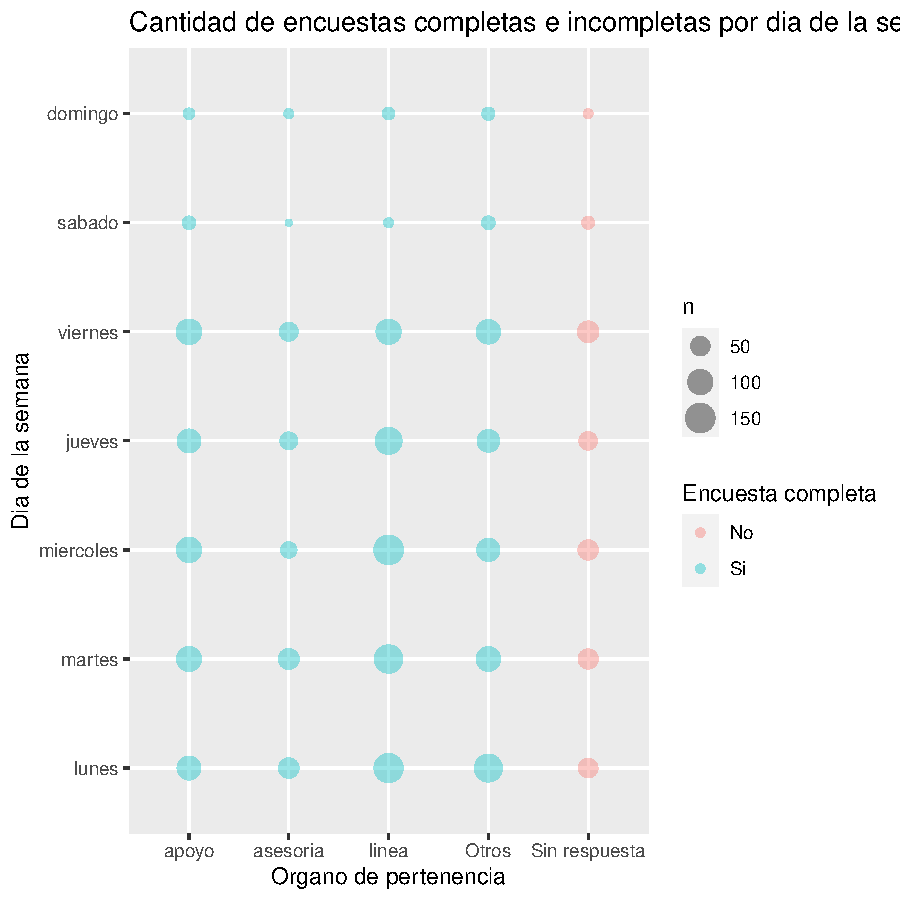
\includegraphics{seguimientov3-021}

Los de organo de linea respondieron poco mas que los demas y en mayor cantidad de lunes a viernes.

\subsection{Cantidad de encuestas completas e incompletas por dia de la semana y sexo}

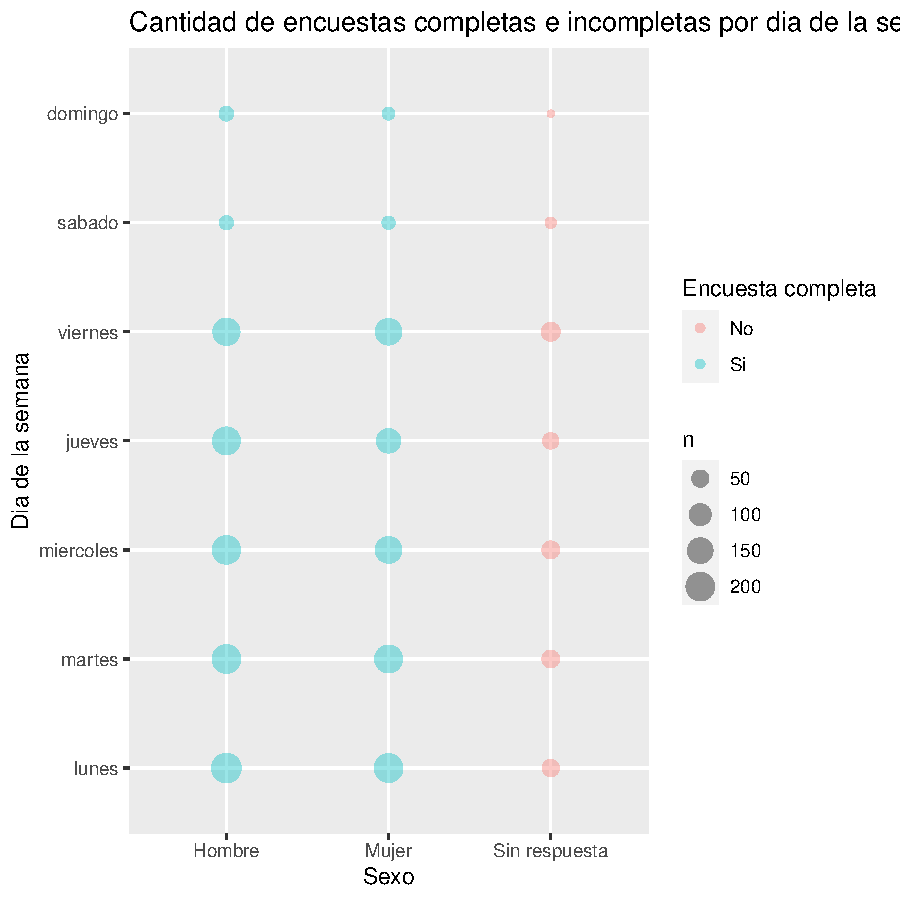
\includegraphics{seguimientov3-022}

Se ve una similar proporcion de respuestas entre los hombres y mujeres todos los dias.

\subsection{Cantidad de encuestas completas e incompletas por dia de la semana y tiempo trabajando en el estado}

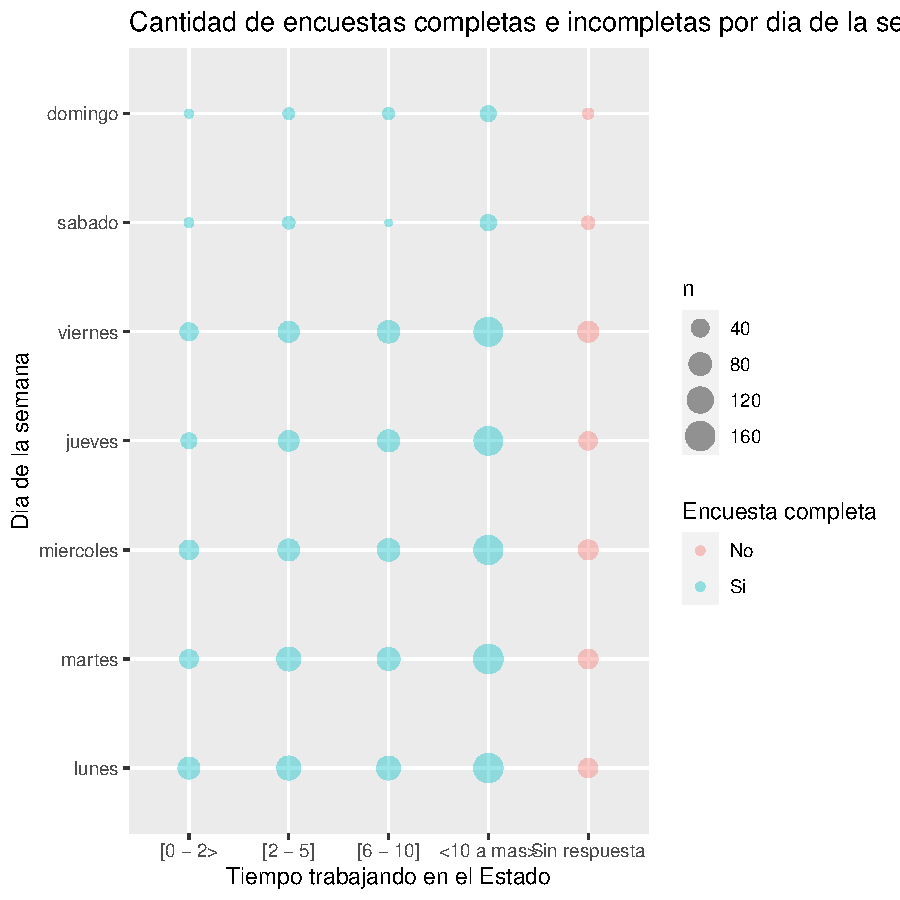
\includegraphics{seguimientov3-023}

Los que tienen de 10 a mas años trabajando fueron los que mayormente respondieron y de lunes a viernes en general.

\subsection{Cantidad de encuestas completas e incompletas por dia de la semana y nivel de gobierno}

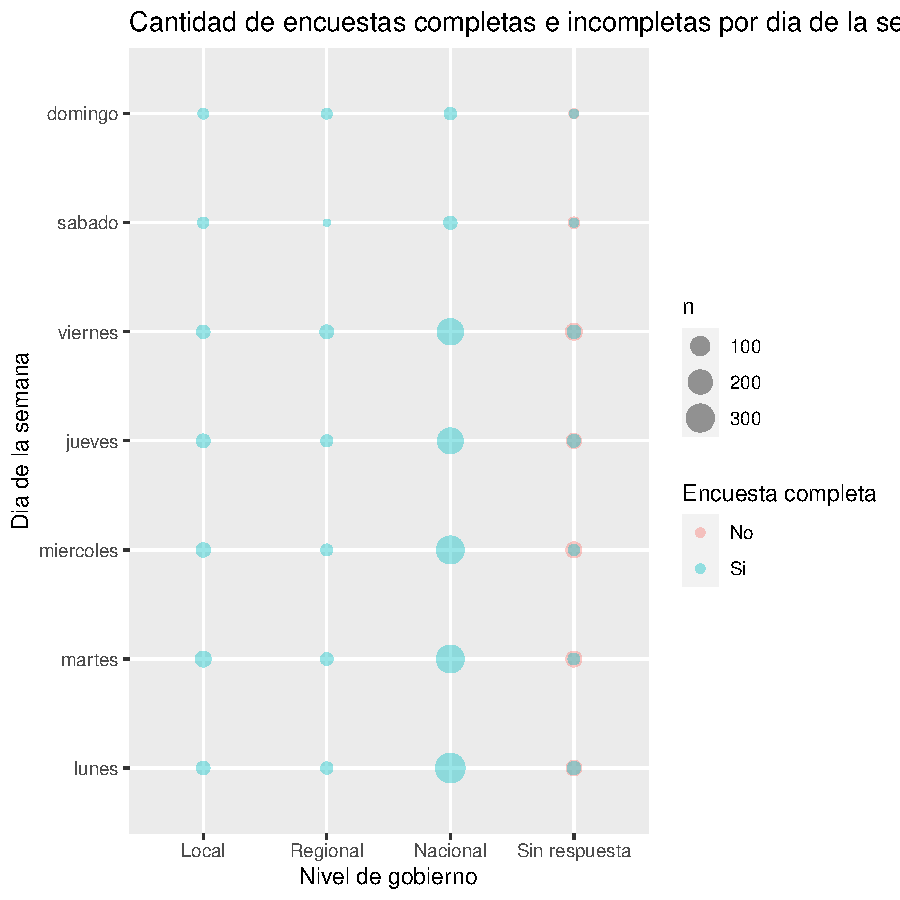
\includegraphics{seguimientov3-024}

De lunes a viernes fueron los dias que se obtuvieron la mayor cantidad de respuestas y fueron de parte del nivel de gobierno nacional.

\subsection{Cantidad de encuestas completas e incompletas por mes y organo de dependencia}

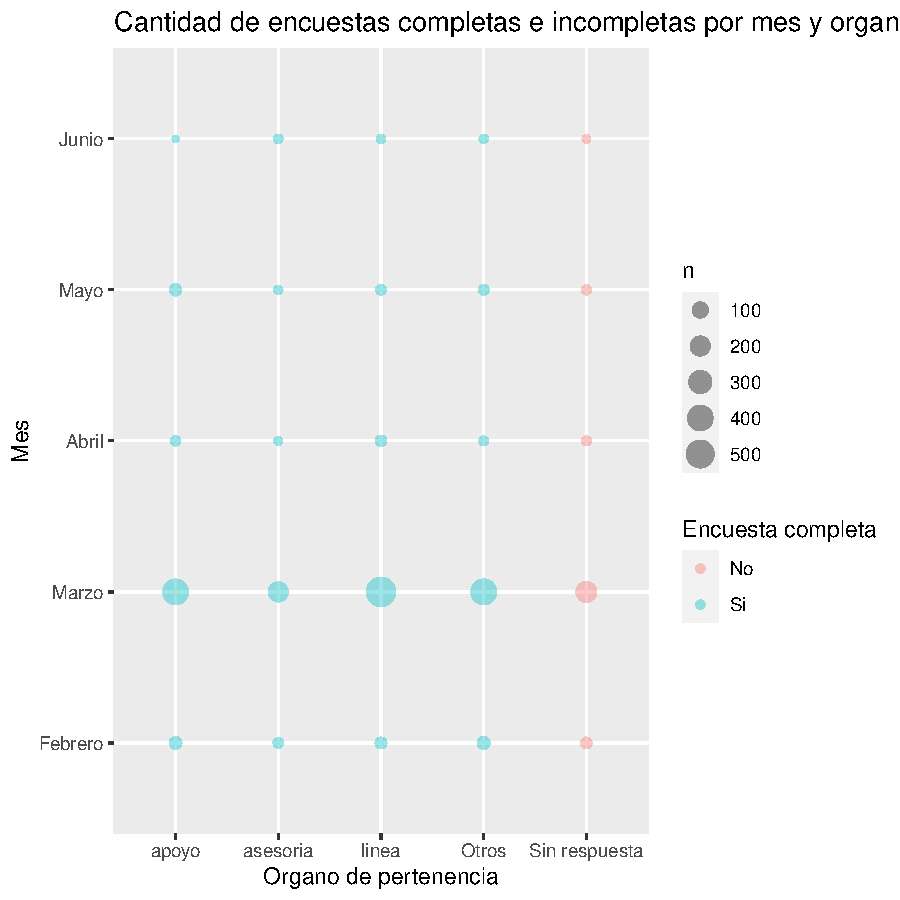
\includegraphics{seguimientov3-025}

Se observa que en marzo se obtuvo la mayor cantidad de respuestas y fue de parte de los de organo de linea.

\subsection{Cantidad de encuestas completas e incompletas por mes y sexo}

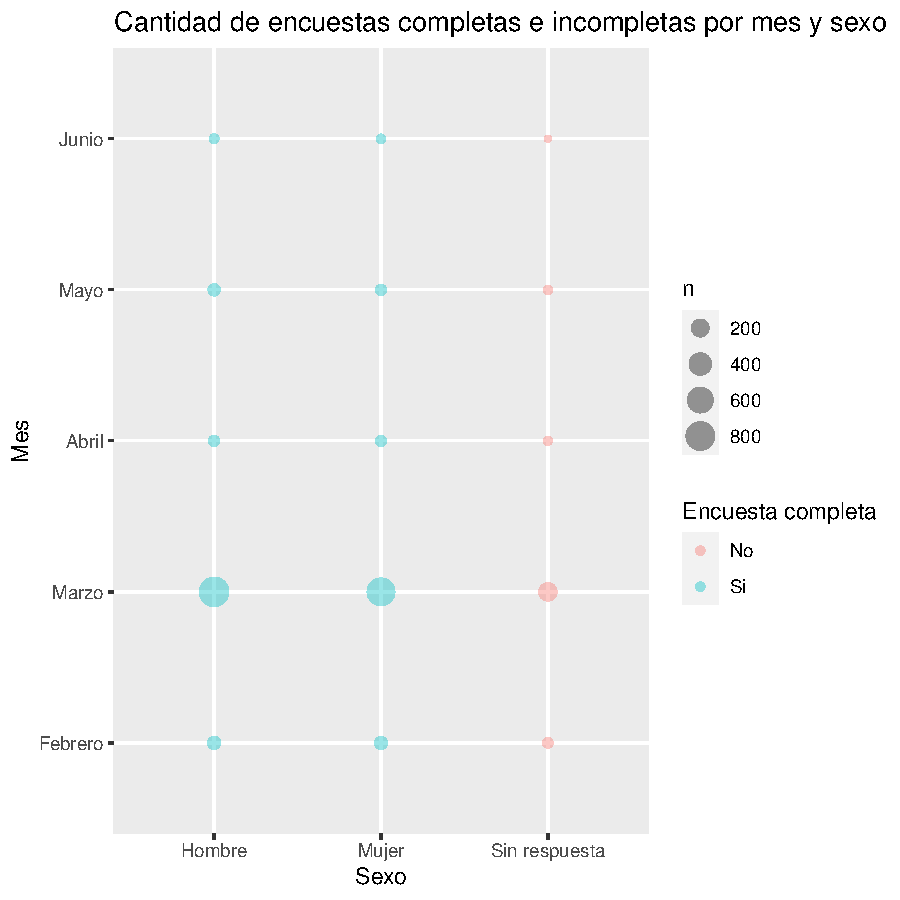
\includegraphics{seguimientov3-026}

La proporcion de las respuestas fue similar a lo largo de los meses entre hombres y mujeres siendo en marzo donde encontramos una mayor cantidad.

\subsection{Cantidad de encuestas completas e incompletas por mes y tiempo trabajando en el estado}

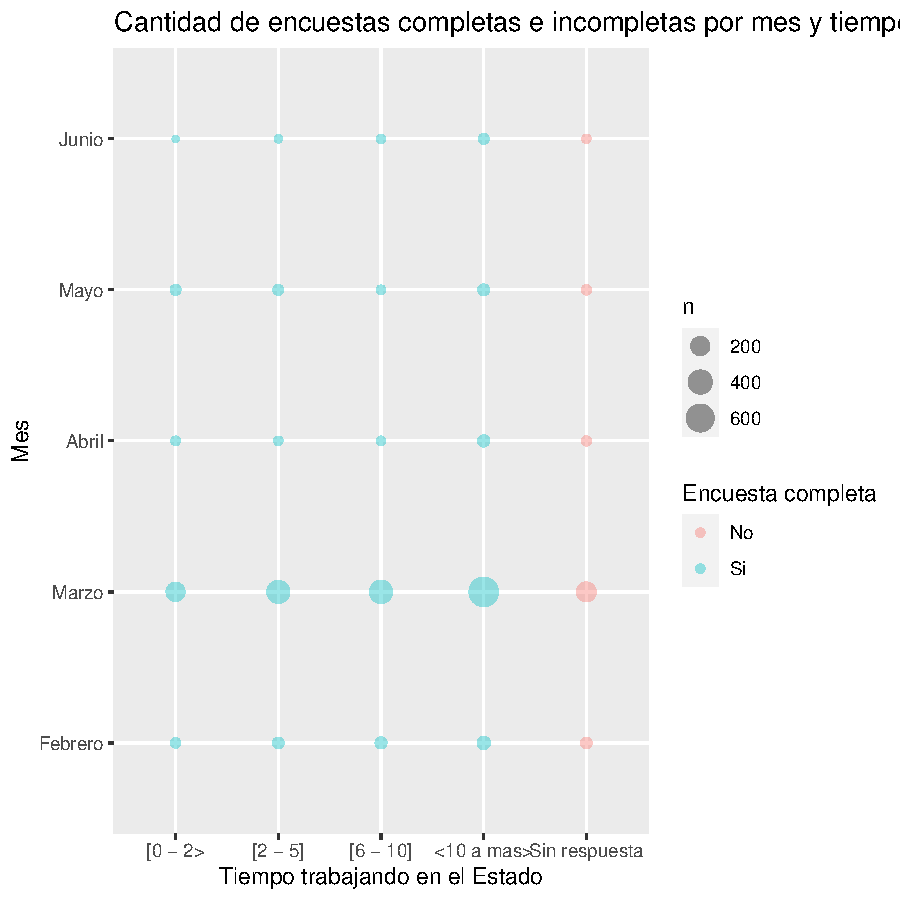
\includegraphics{seguimientov3-027}

En marzo se obtuvo la mayor cantidad de encuestas respondidas siendo los que trabajaron de 10 a mas años los que mas respondieron.

\subsection{Cantidad de encuestas completas e incompletas por mes y nivel de gobierno}

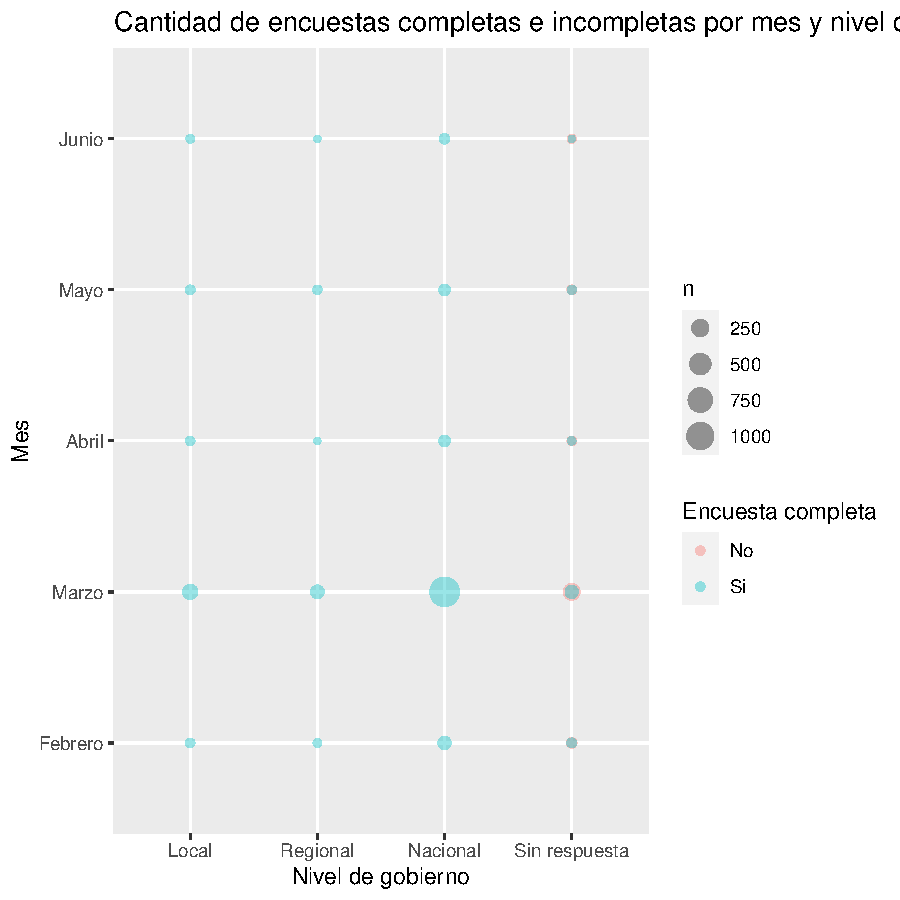
\includegraphics{seguimientov3-028}

Se obtuvo la mayor cantidad de respuestas de los de nivel de gobierno nacional y en marzo.

\subsection{Cantidad de encuestas completas e incompletas por organo de pertenencia y sexo}

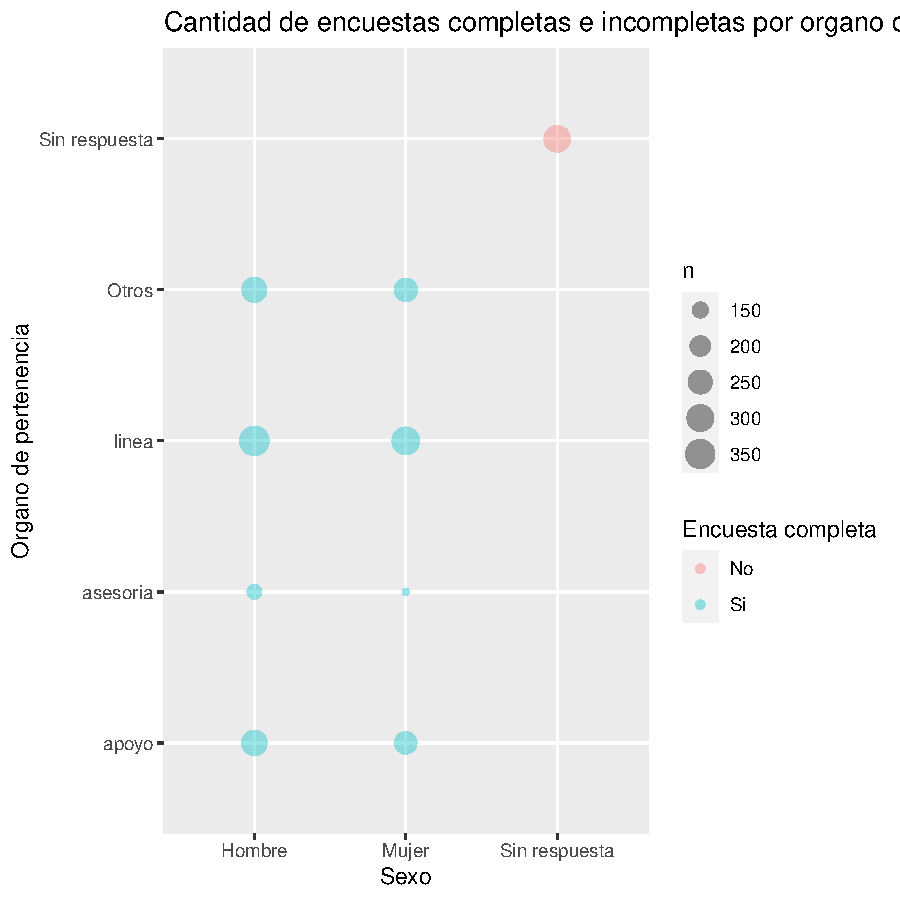
\includegraphics{seguimientov3-029}

Hay una similar proporcion de respuestas entre los hombres y las mujeres alrededor de los organos de pertenencia.

\subsection{Cantidad de encuestas completas e incompletas por organo de pertenencia y tiempo trabajando en el estado}

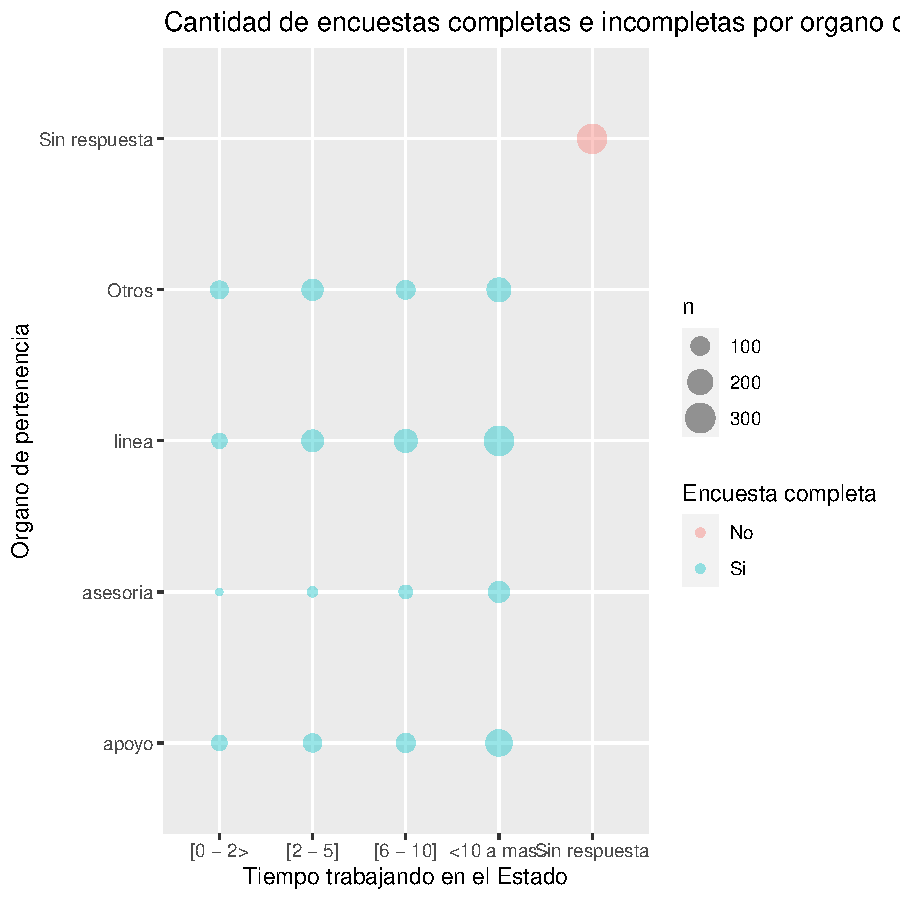
\includegraphics{seguimientov3-030}

Se observa que va aumentando la cantidad de respuestas de los organos de pertenencia a traves del tiempo trabajando en el estado.

\subsection{Cantidad de encuestas completas e incompletas por organo de pertenencia y nivel de gobierno}

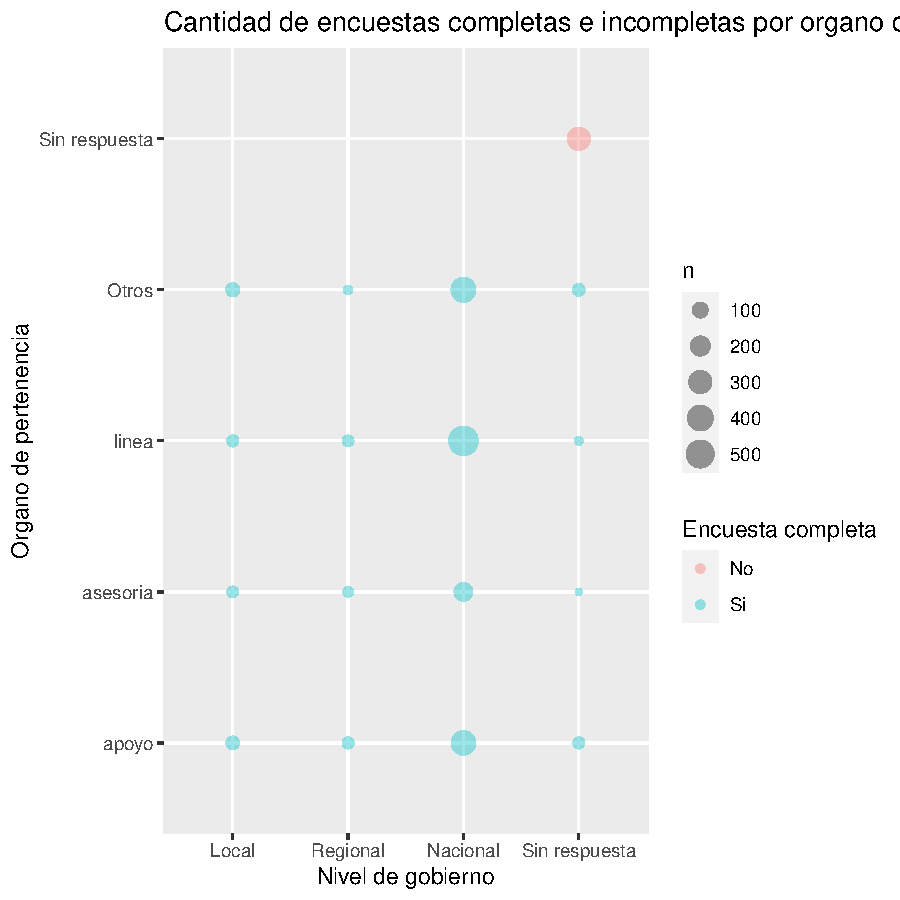
\includegraphics{seguimientov3-031}

En el grafico a manera exploratoria se observa que obtuvimos mas respuestas de los que pertenecen al nivel de gobierno nacional independientemente de a que organo de pertenencia este.

\section{Panorama antes del covid: 28 de febrero hasta el 15 de marzo }

\begin{Schunk}
\begin{Sinput}
> 
> # 1902 observaciones = 85.10% del total
> 
\end{Sinput}
\end{Schunk}


\begin{Schunk}
\begin{Soutput}
Rows: 1,902
Columns: 10
$ Fecha                            <dttm> 2020-03-15, 2020-03-15, 2020-03-1...
$ Hora                             <dbl> 22, 22, 22, 18, 18, 17, 17, 17, 15...
$ Dia                              <dbl> 15, 15, 15, 15, 15, 15, 15, 15, 15...
$ `Dia de la semana`               <fct> domingo, domingo, domingo, domingo...
$ Mes                              <fct> Marzo, Marzo, Marzo, Marzo, Marzo,...
$ `Organo de pertenencia`          <fct> Otros, apoyo, asesoria, Otros, Otr...
$ Sexo                             <chr> "Mujer", "Mujer", "Hombre", "Mujer...
$ `Tiempo trabajando en el Estado` <fct> [2 - 5], [6 - 10], <10 a mas>, <10...
$ `Nivel de gobierno`              <fct> Sin respuesta, Local, Local, Local...
$ `Encuesta completa`              <chr> "Si", "Si", "Si", "Si", "Si", "Si"...
\end{Soutput}
\end{Schunk}


\subsection{Cantidad de encuestas completas e incompletas por fecha y Hora}

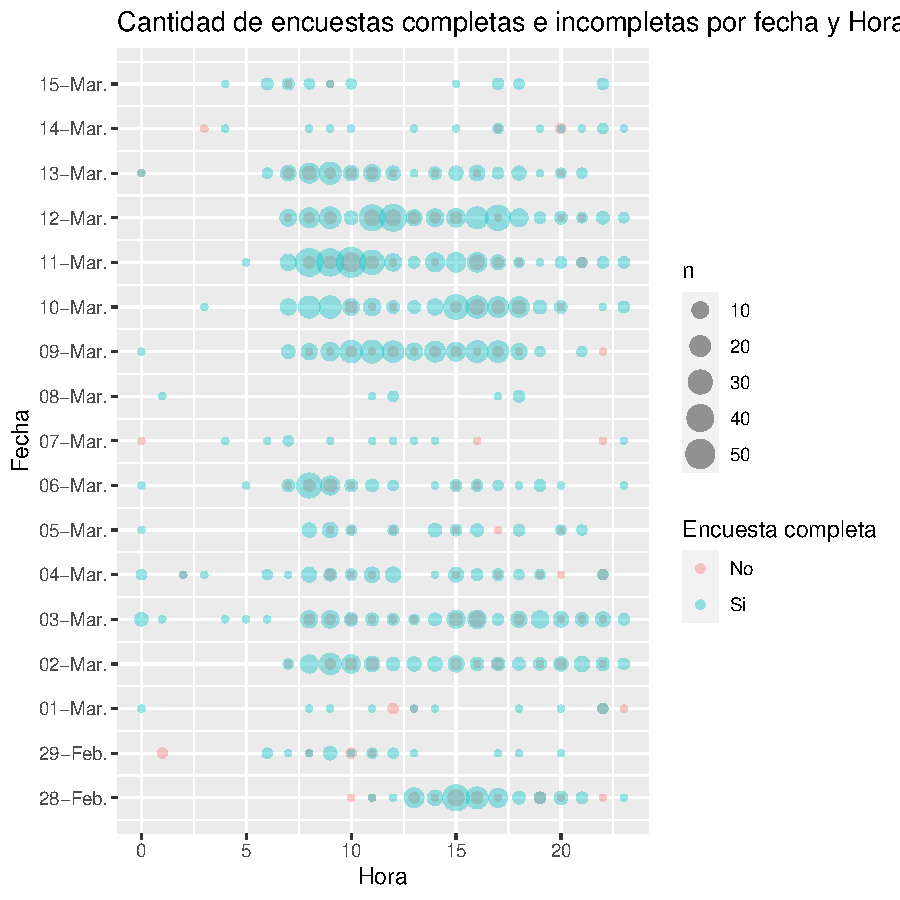
\includegraphics{seguimientov3-034}

Se puede apreciar que hubo mayor recepcion de encuestas diarias entre el 9 y 13 de Marzo y en horario de trabajo.

\subsection{Cantidad de encuestas completas e incompletas por fecha y organo de pertenencia}

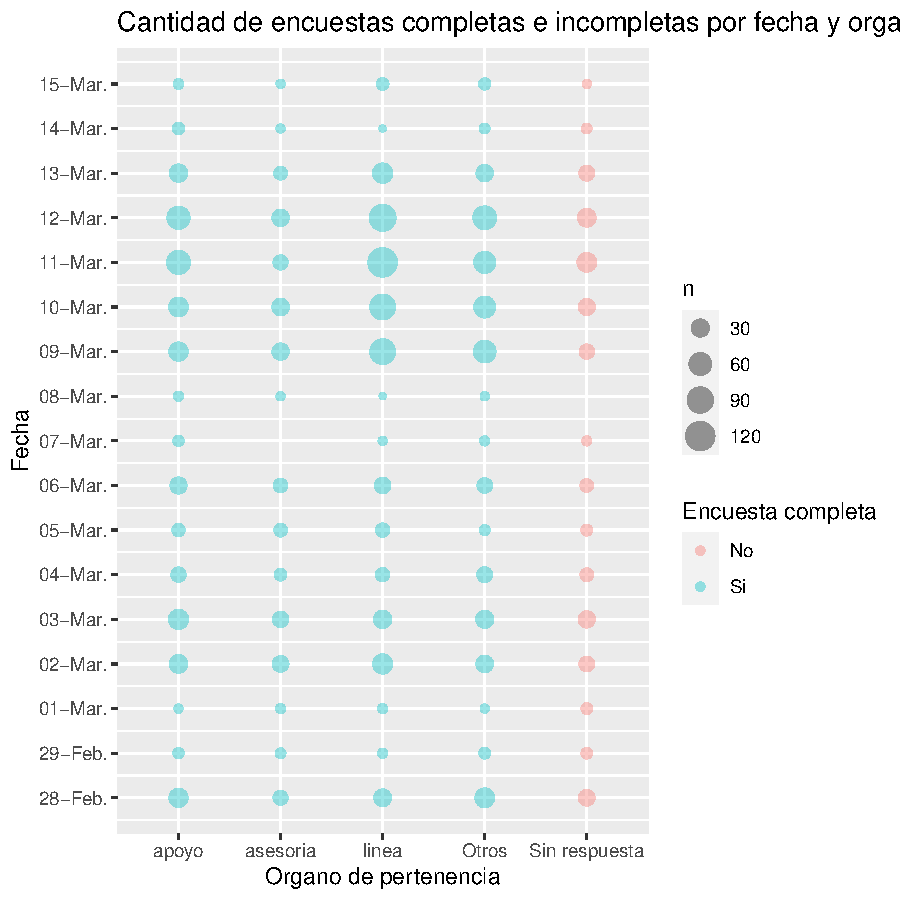
\includegraphics{seguimientov3-035}

Vemos graficamente que los de organo de linea fueron los que mas contestaban entre el 9 y 13 de marzo.

\subsection{Cantidad de encuestas completas e incompletas por fecha y sexo}

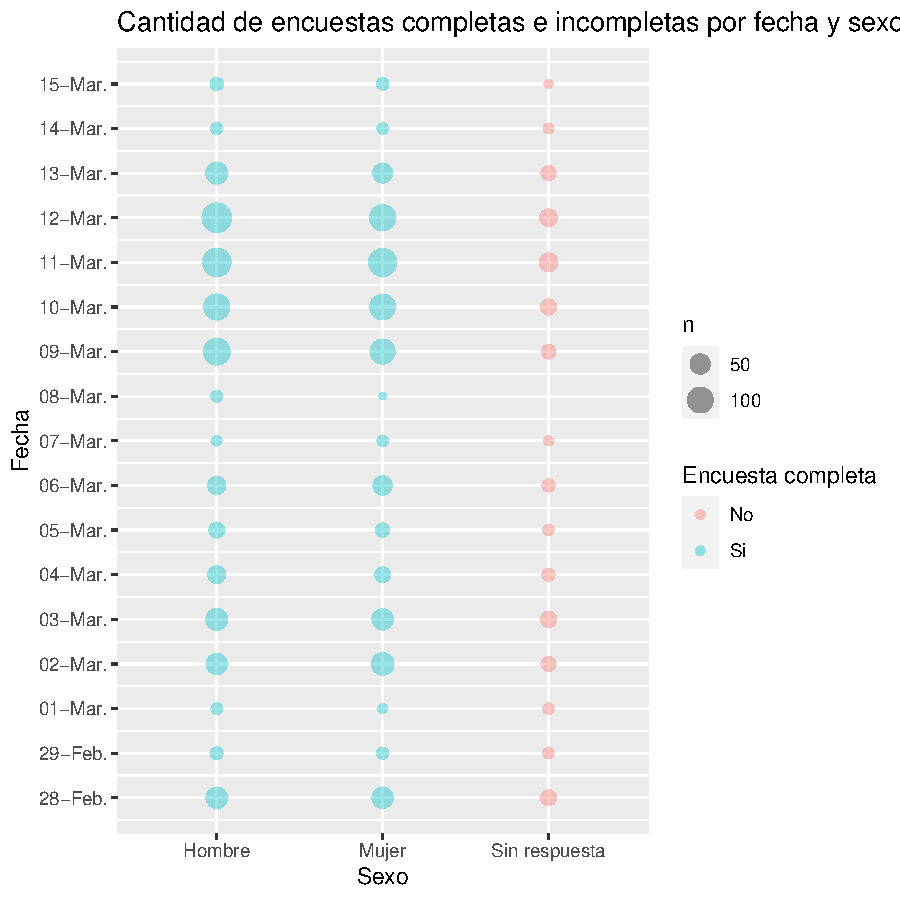
\includegraphics{seguimientov3-036}

La proporcion de respuestas entre hombre y mujeres se ve similar en todo el periodo y obtuvimos mayores resultados entre el 9 y 13 de marzo.

\subsection{Cantidad de encuestas completas e incompletas por fecha y tiempo trabajando en el estado}

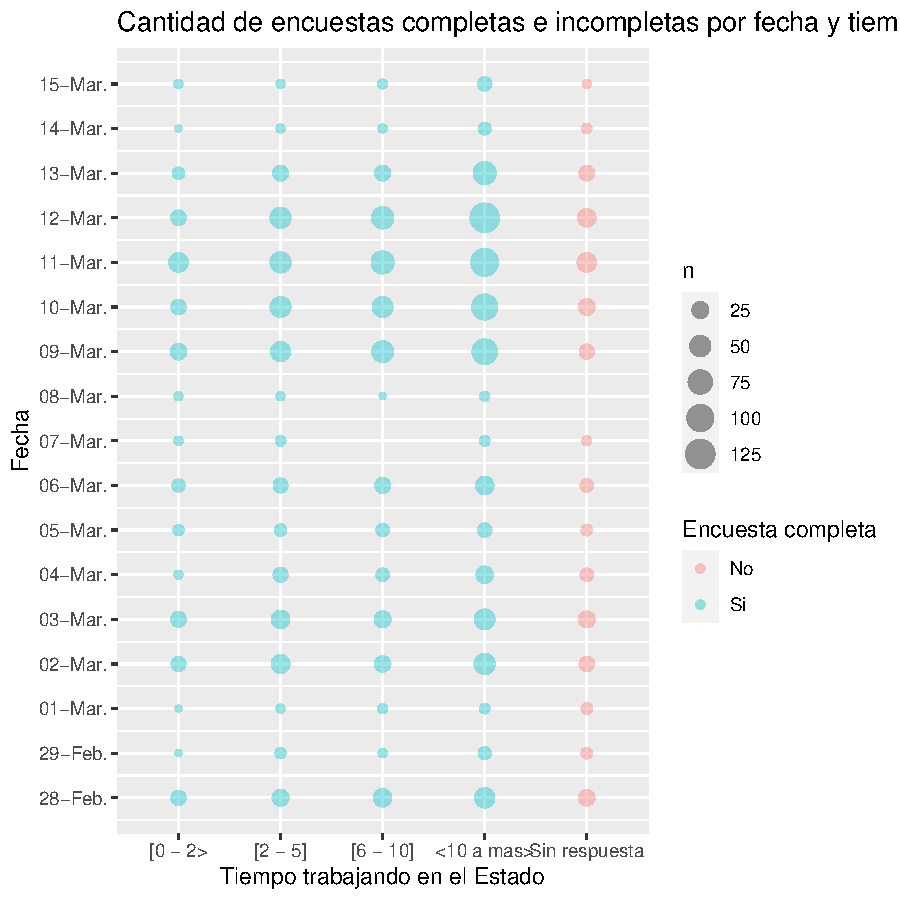
\includegraphics{seguimientov3-037}

Entre el 9 y 13 de marzo habian respondido en mayor numero a las encuestas los que estan trabajando de 10 años a mas.

\subsection{Cantidad de encuestas completas e incompletas por fecha y nivel de gobierno}

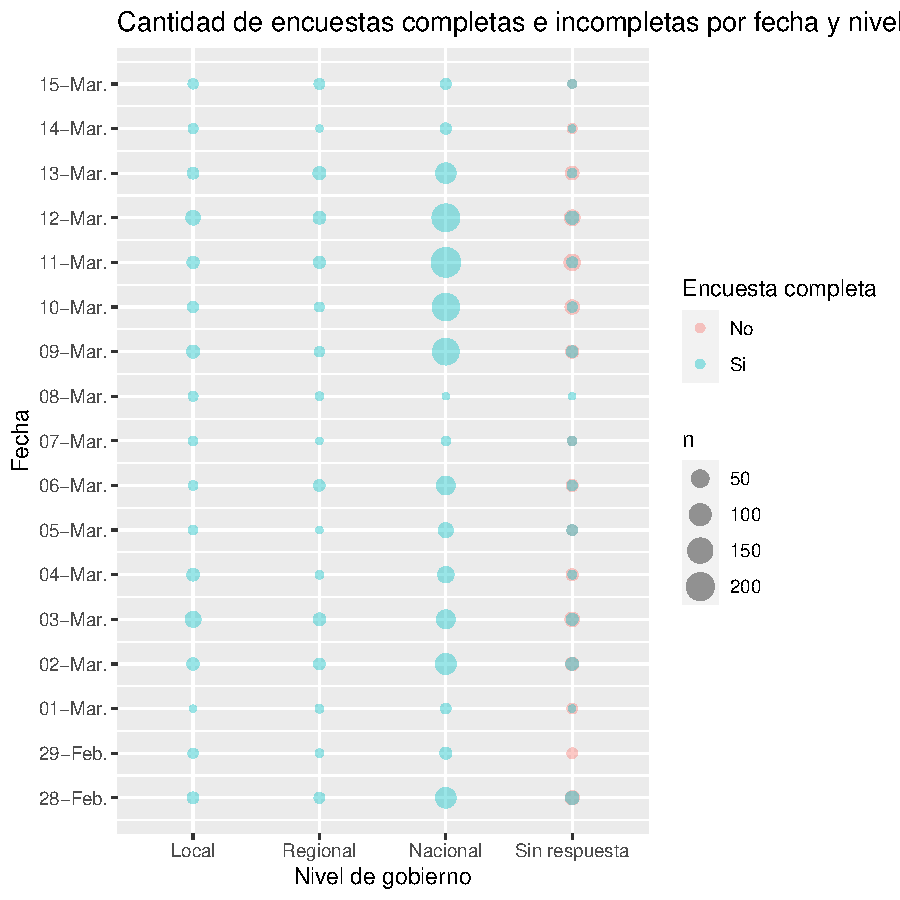
\includegraphics{seguimientov3-038}

Entre el 9 y 13 de marzo obtuvimos mayores cantidades de respuestas del nivel de gobierno Nacional.

\subsection{Cantidad de encuestas completas e incompletas por hora y dia}

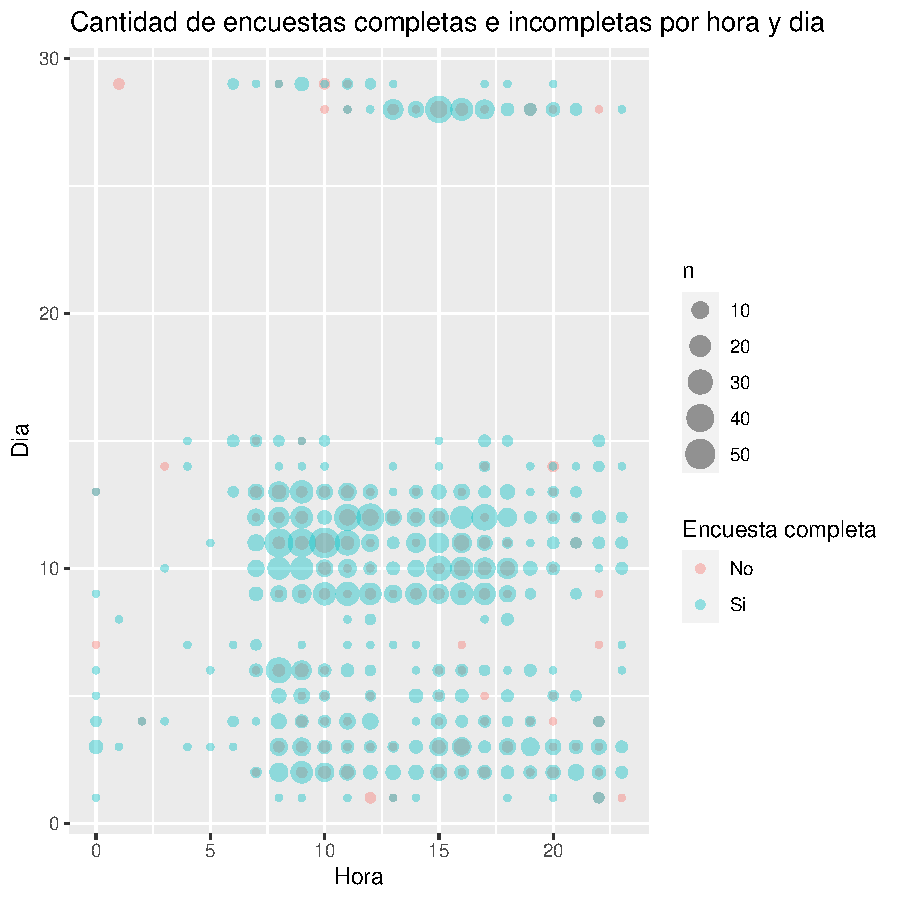
\includegraphics{seguimientov3-039}

Se podria decir que respondian las encuestas generalmene en el horario de trabajo y antes de la quincena de mes.

\subsection{Cantidad de encuestas completas e incompletas por hora y dia de la semana}

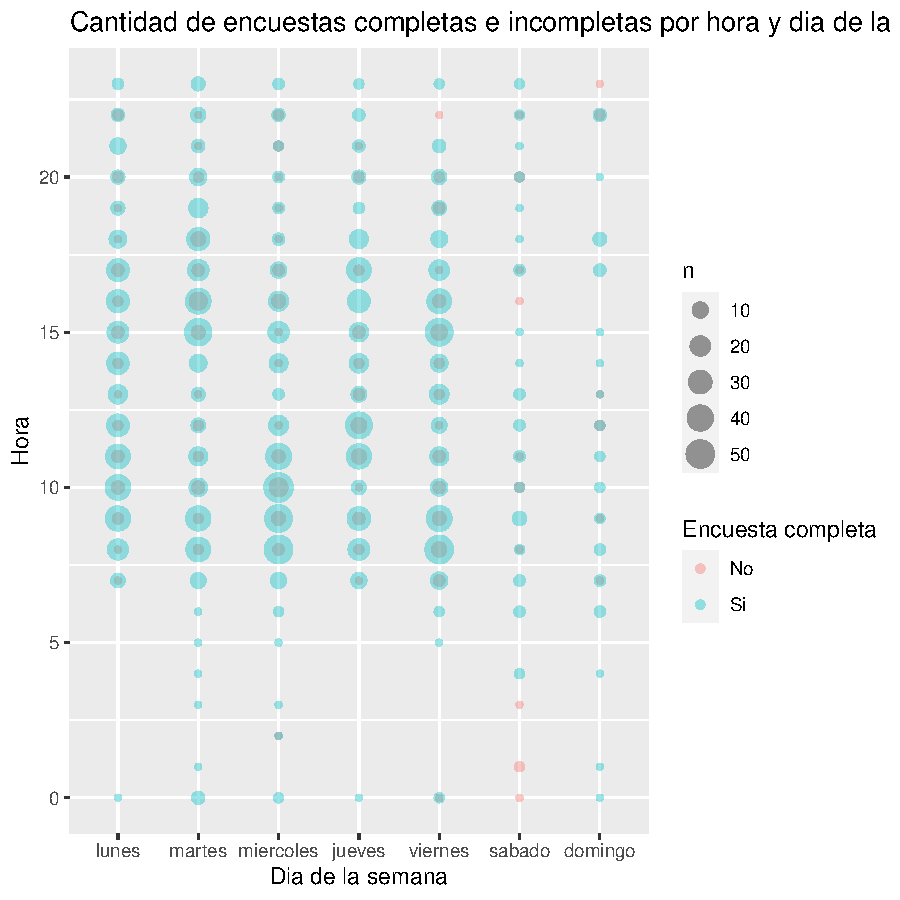
\includegraphics{seguimientov3-040}

En este grafico se aprecia mejor que mayormente respondieron a las encuestas en las horas de trabajo y en dias laborales de lunes a viernes.

\subsection{Cantidad de encuestas completas e incompletas por hora y mes}

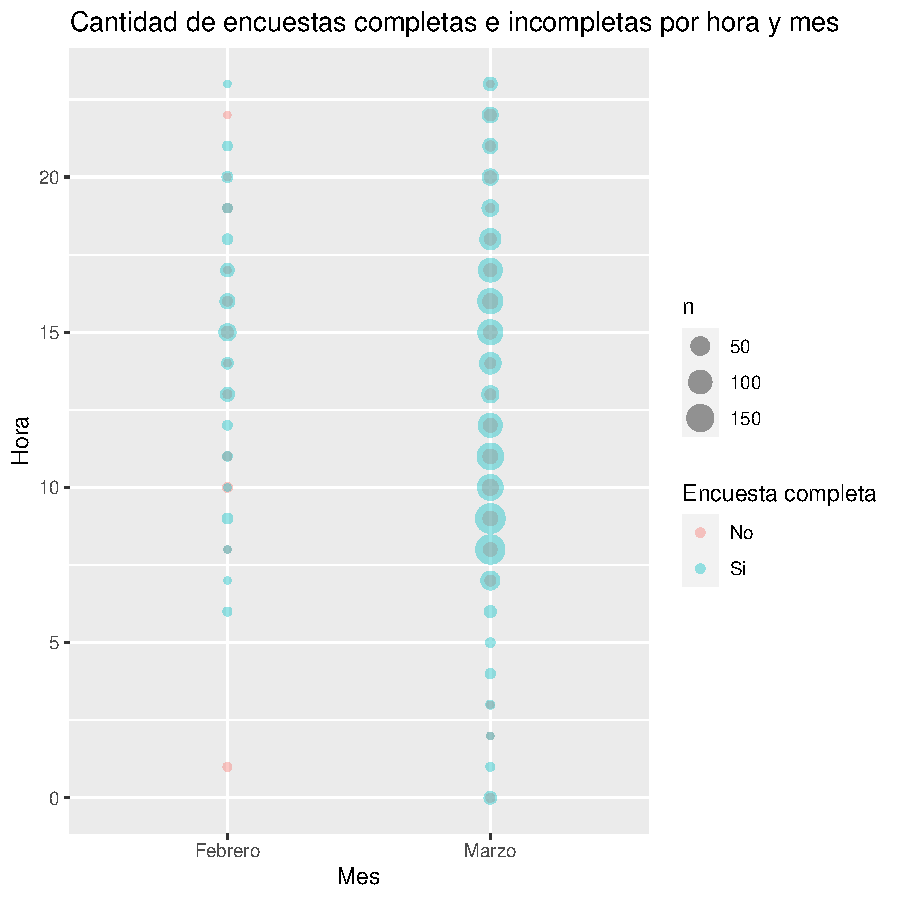
\includegraphics{seguimientov3-041}

En marzo es donde se obtubo mayor cantidad de respuestas en horarios laborales.

\subsection{Cantidad de encuestas completas e incompletas por hora y organo de pertenencia}

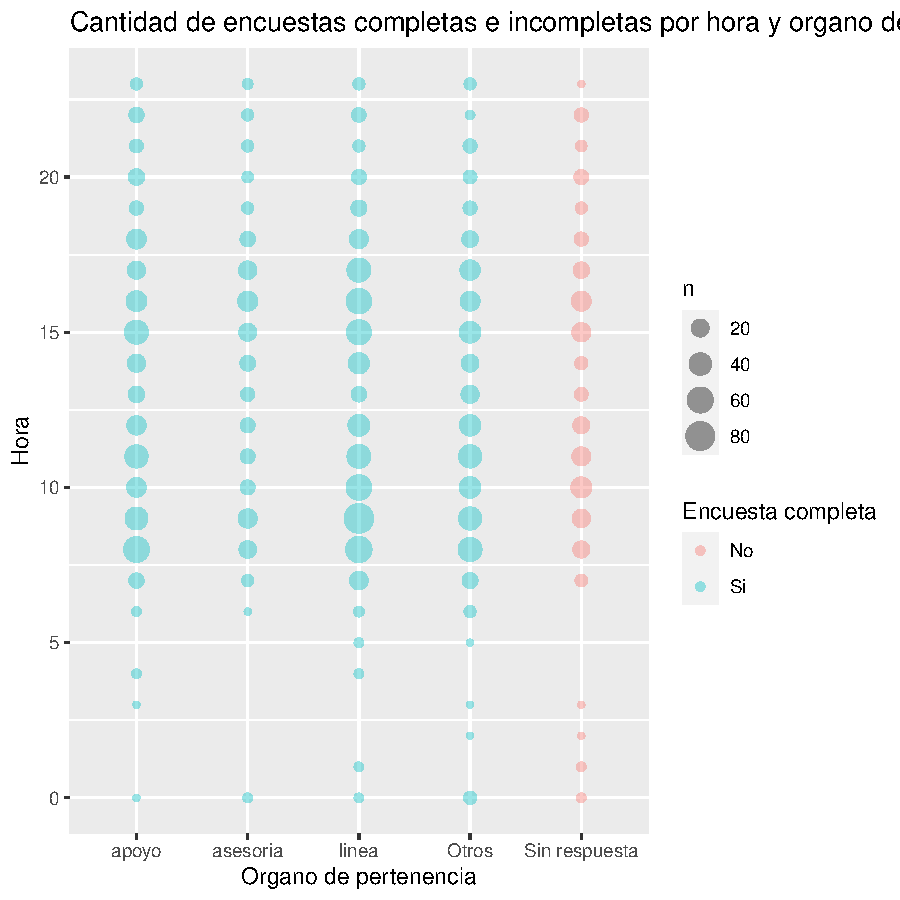
\includegraphics{seguimientov3-042}

A lo largo de las horas laborales los de organo de linea respondieron un poco mas con respecto a los demas.

\subsection{Cantidad de encuestas completas e incompletas por hora y sexo}

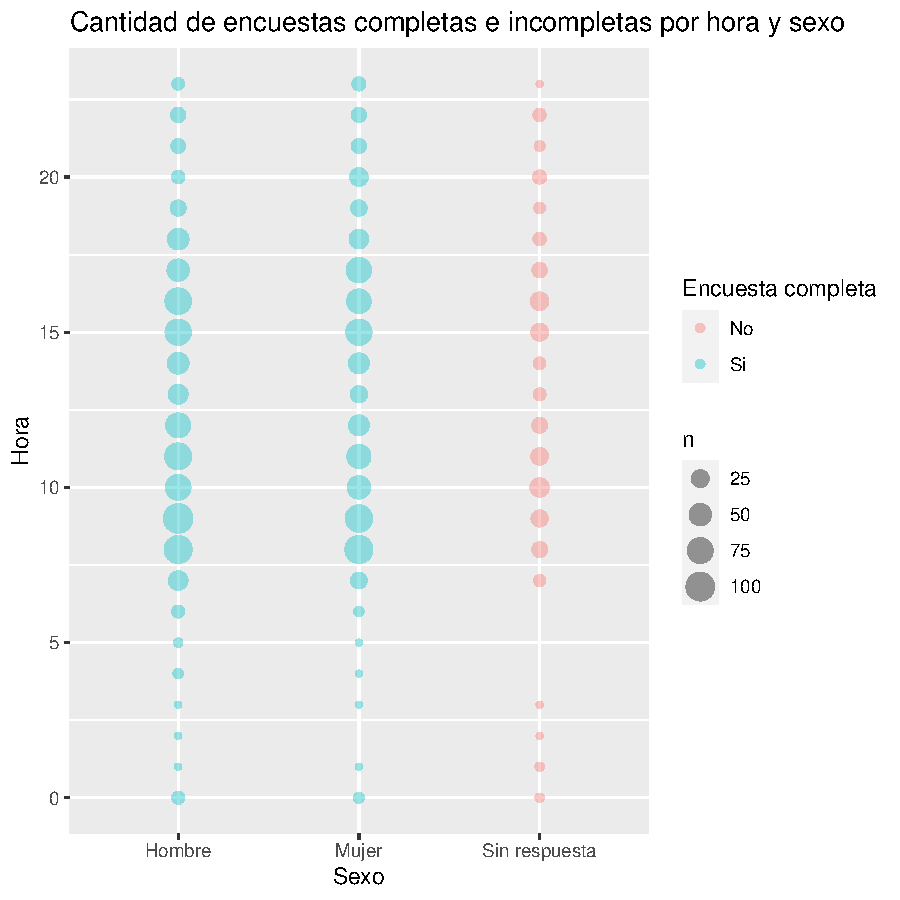
\includegraphics{seguimientov3-043}

Los hombres y las mujeres contestaron en similar proporcion y se obtuvieron mas respuestas de ambos en las horas laborales.

\subsection{Cantidad de encuestas completas e incompletas por hora y tiempo trabajando en el estado}

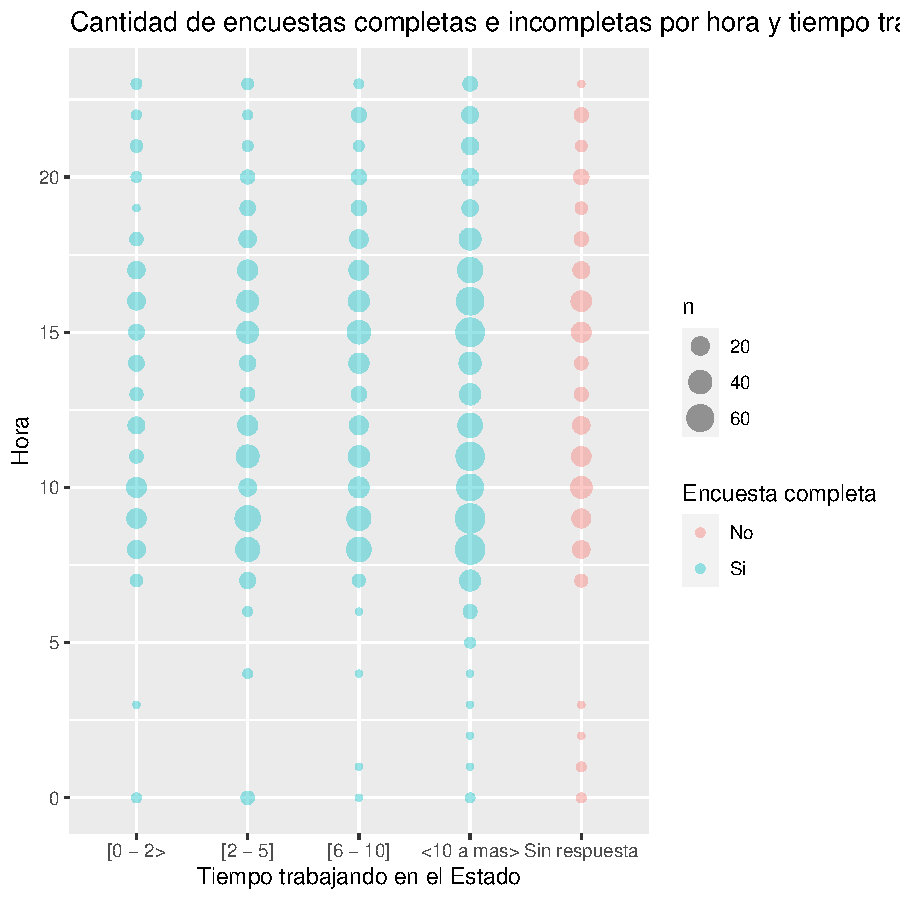
\includegraphics{seguimientov3-044}

Los que mas respondieron fueron los que trabajaron de 10 años a mas y durante el horario laboral.

\subsection{Cantidad de encuestas completas e incompletas por hora y nivel de gobierno}

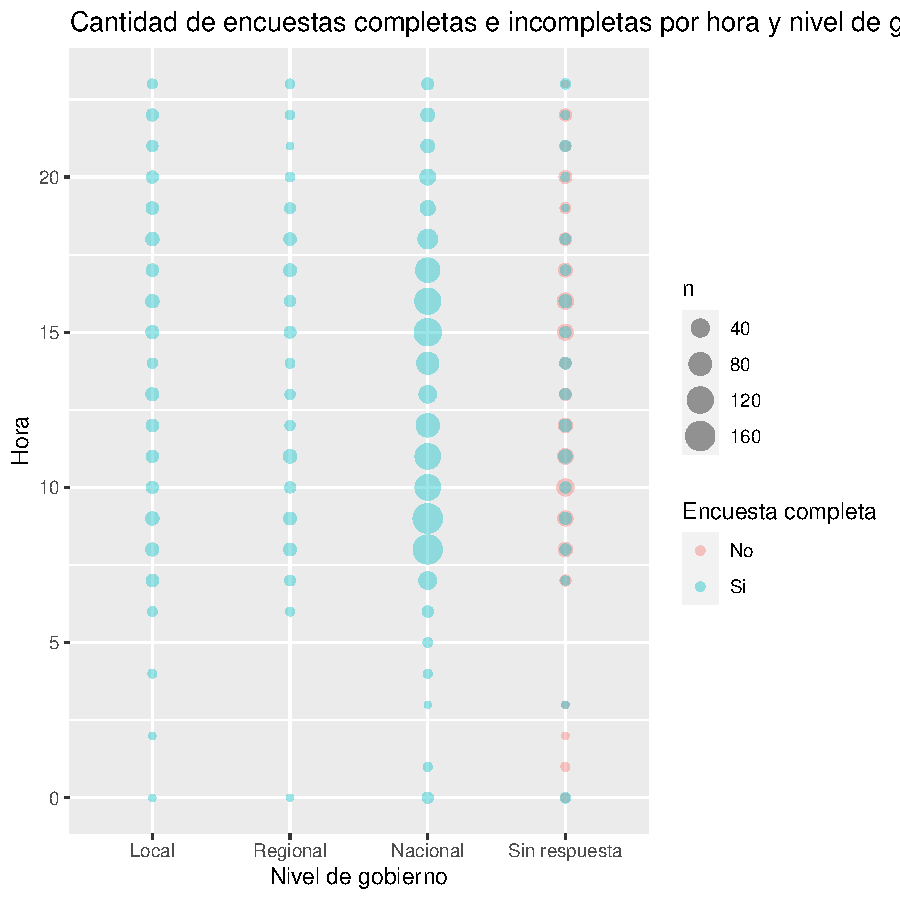
\includegraphics{seguimientov3-045}

Los de nivel de gobierno nacional fueron los que respondieron en mayor cantidad y en horario laboral.

\subsection{Cantidad de encuestas completas e incompletas por dia y mes}

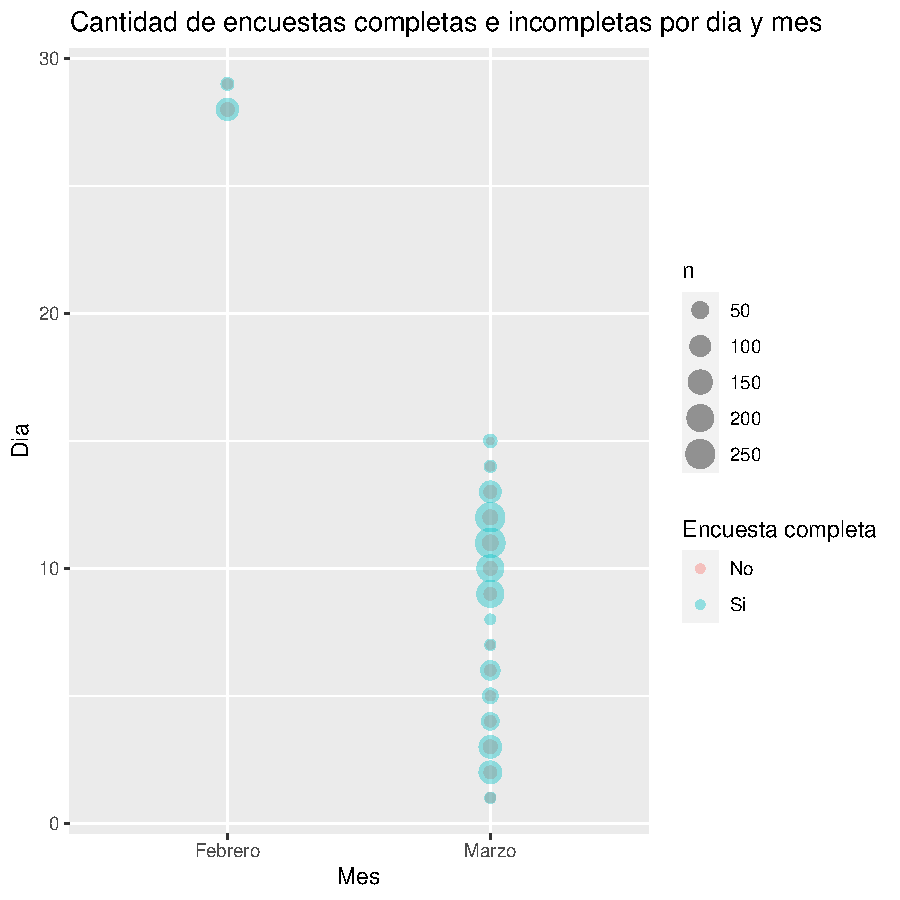
\includegraphics{seguimientov3-046}

Entre el 9 y 13 de marzo se recopilaron la gran mayoria de encuestas.

\subsection{Cantidad de encuestas completas e incompletas por dia y organo de pertenencia}

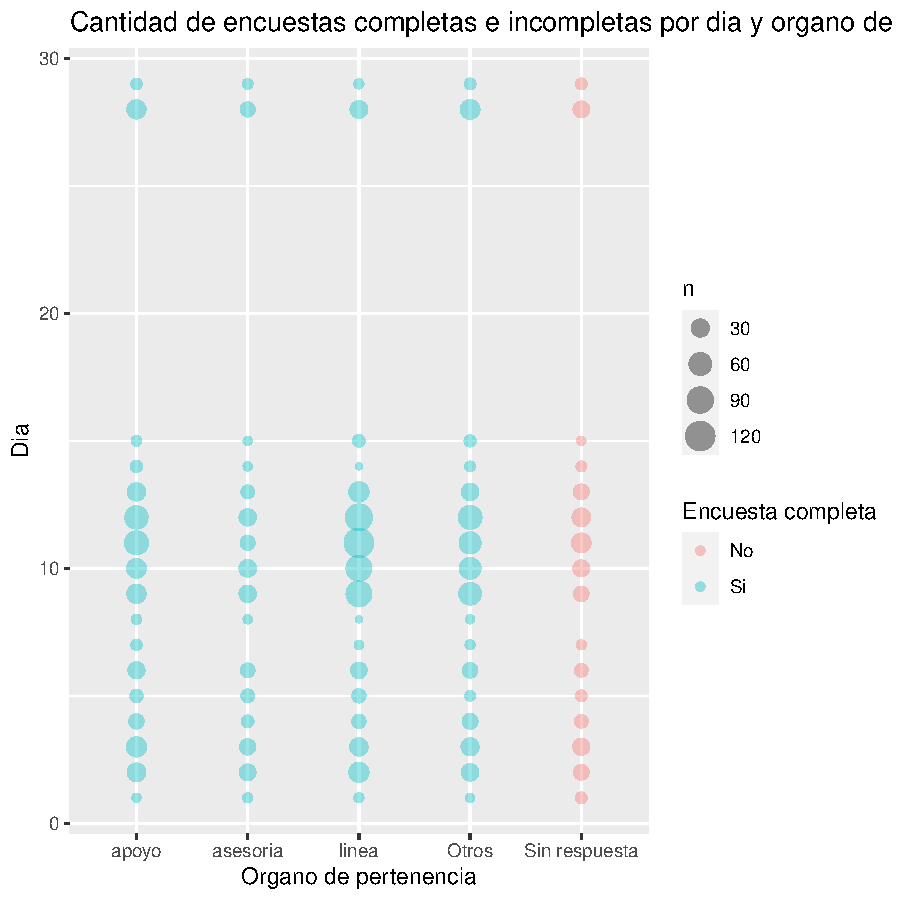
\includegraphics{seguimientov3-047}

Los de organo de linea fueron los que mas contestaron y lo hicieron generalmente alrededor del dia 10.

\subsection{Cantidad de encuestas completas e incompletas por dia y sexo}

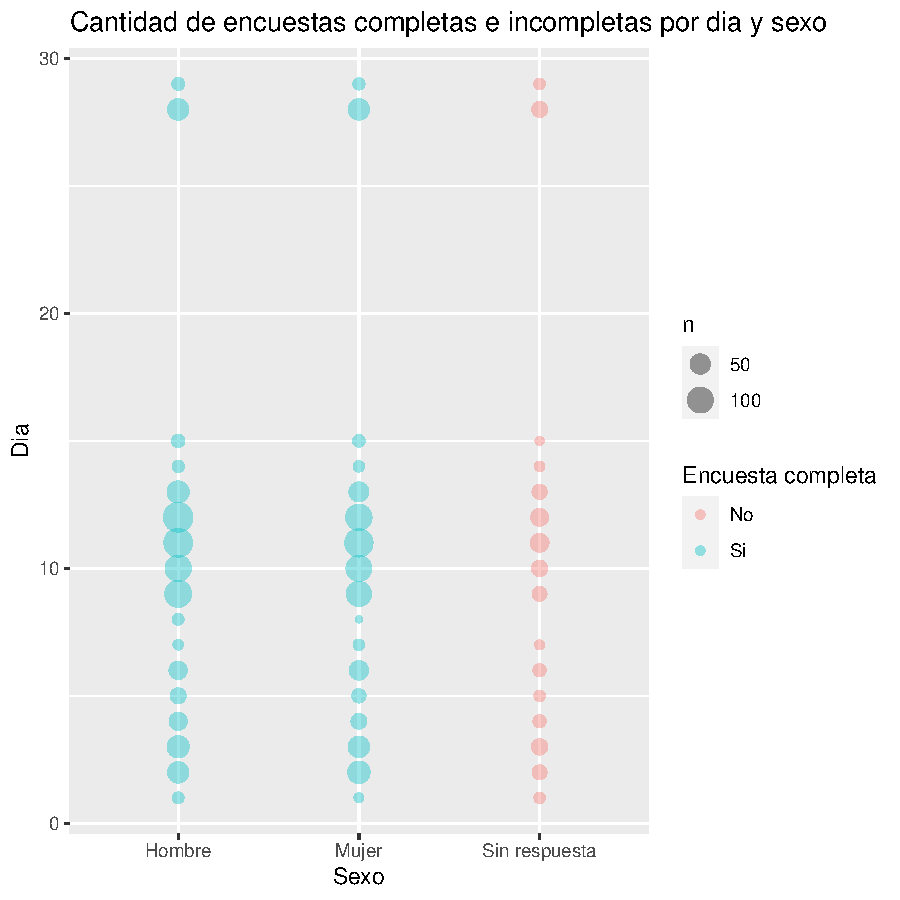
\includegraphics{seguimientov3-048}

La cantidad de encuestas recopiladas por hombres y mujeres fueron similares y de mayor cantidad alrededor del dia 10.

\subsection{Cantidad de encuestas completas e incompletas por dia y tiempo trabajando en el estado}

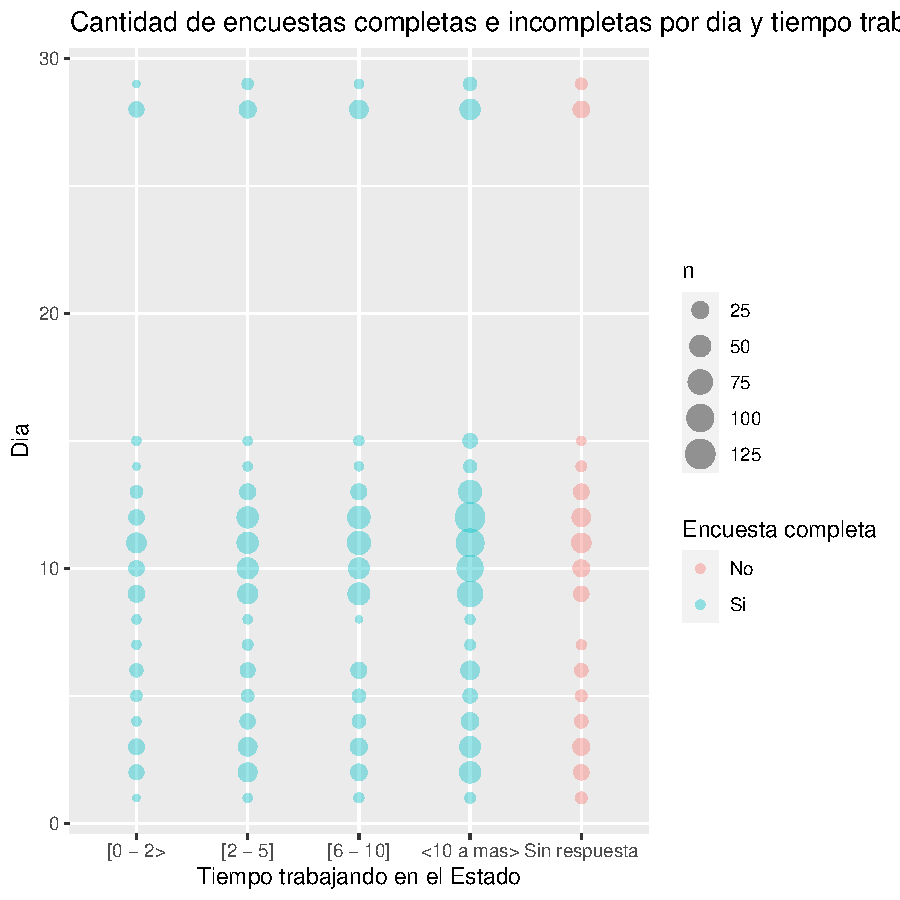
\includegraphics{seguimientov3-049}

Los que tienen de 10 a mas años trabajando en el estado fueron los que mas respondieron y alrededor del dia 10.

\subsection{Cantidad de encuestas completas e incompletas por dia y nivel de gobierno}

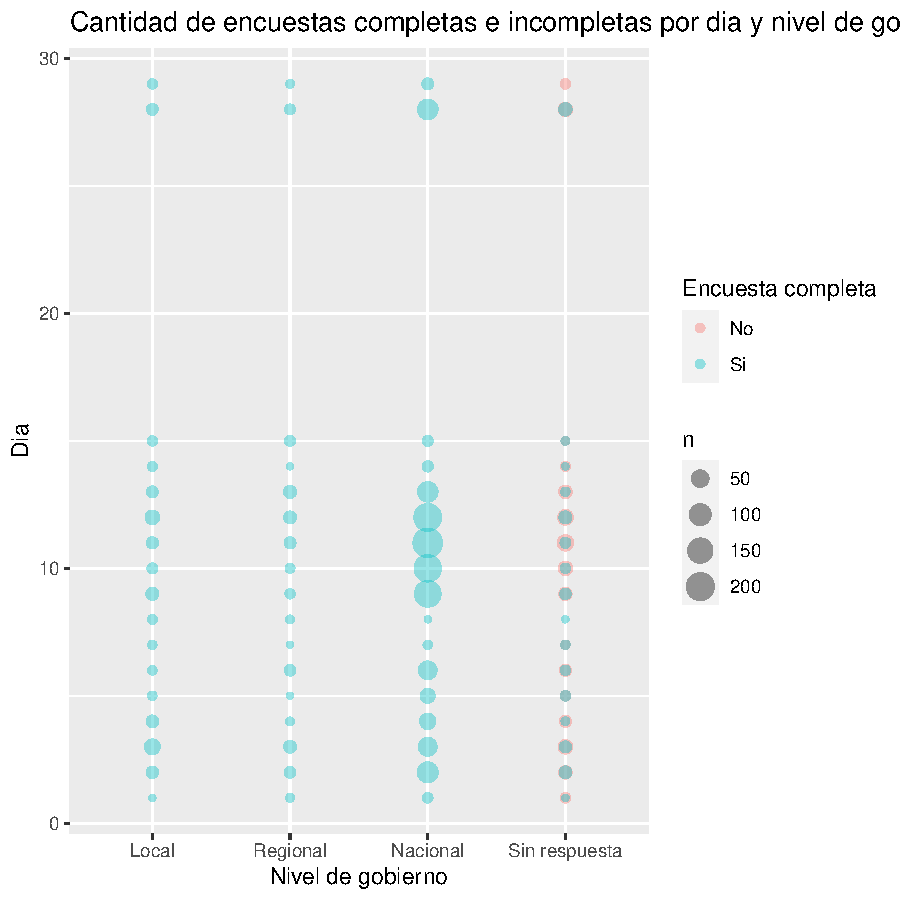
\includegraphics{seguimientov3-050}

Hubo mayor recepcion de respuestas departe del nivel de gobierno nacional y lo hicieron mayormente alrededor del dia 10.

\subsection{Cantidad de encuestas completas e incompletas por dia de la semana y mes}

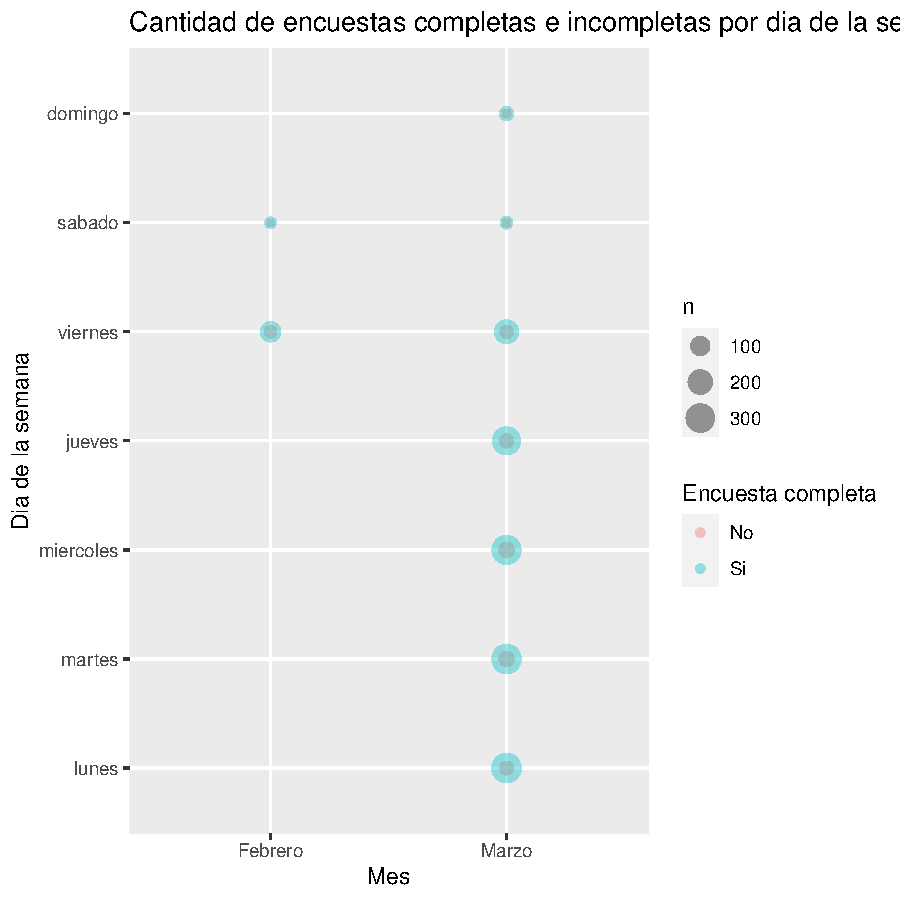
\includegraphics{seguimientov3-051}

Fue en Marzo y de lunes a viernes donde se obtuvo la mayor cantidad de respuestas.

\subsection{Cantidad de encuestas completas e incompletas por dia de la semana y organo de pertenencia}

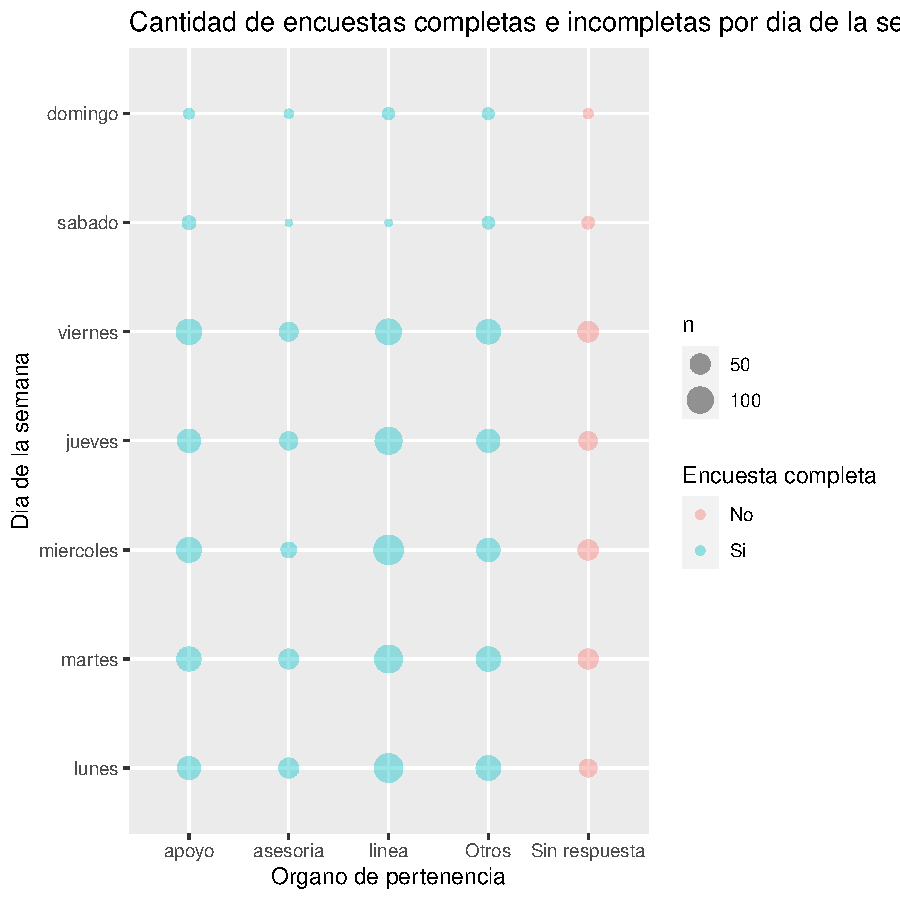
\includegraphics{seguimientov3-052}

Los de organo de linea respondieron poco mas que los demas y en mayor cantidad de lunes a viernes.

\subsection{Cantidad de encuestas completas e incompletas por dia de la semana y sexo}

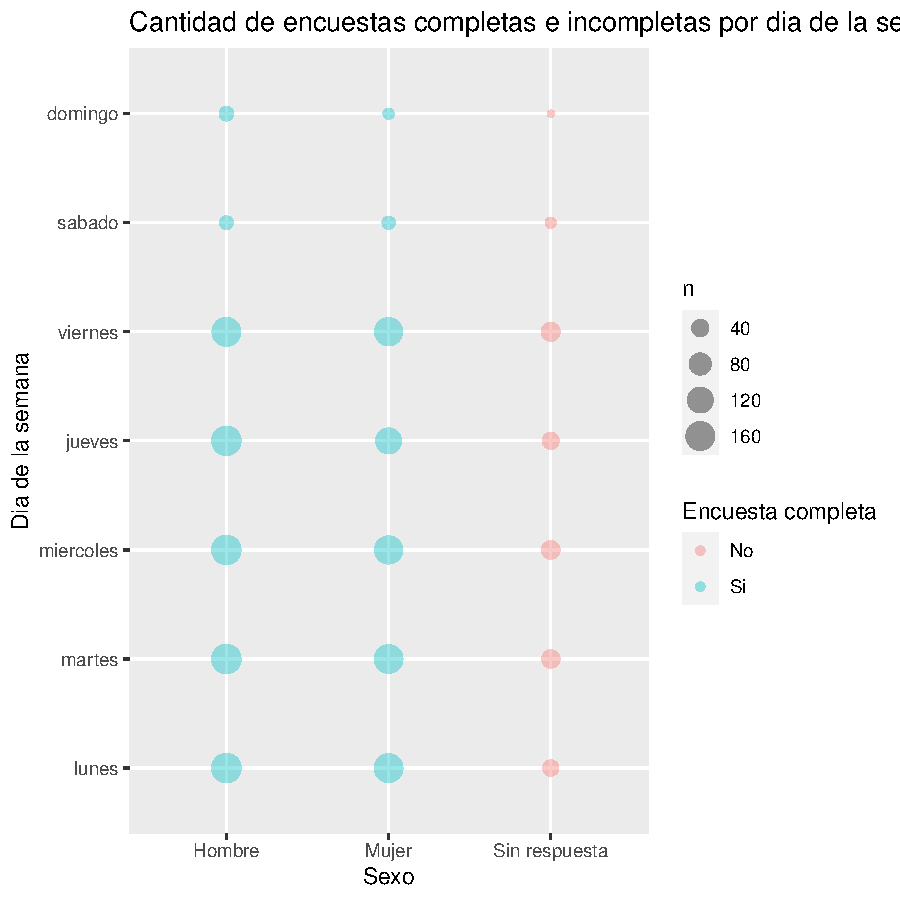
\includegraphics{seguimientov3-053}

Se ve una similar proporcion de respuestas entre los hombres y mujeres todos los dias siendo los dias laborales donde mas responden.

\subsection{Cantidad de encuestas completas e incompletas por dia de la semana y tiempo trabajando en el estado}

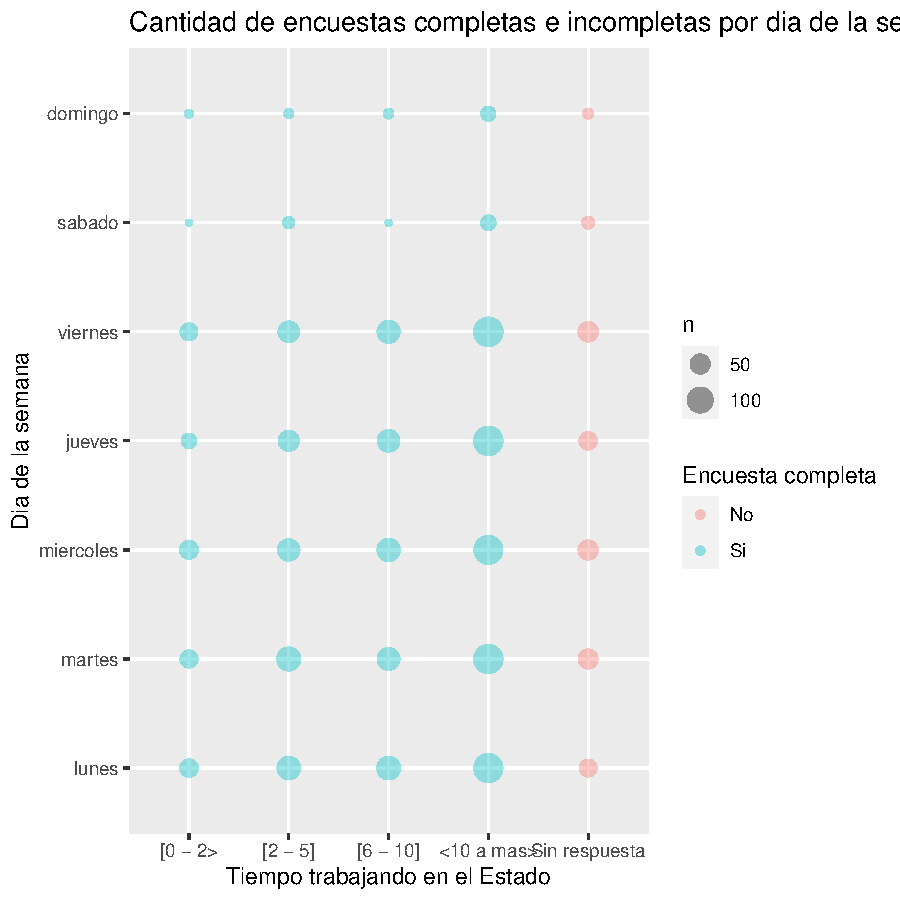
\includegraphics{seguimientov3-054}

Los que tienen de 10 a mas años trabajando fueron los que mayormente respondieron y de lunes a viernes en general.

\subsection{Cantidad de encuestas completas e incompletas por dia de la semana y nivel de gobierno}

\includegraphics{seguimientov3-055}

De lunes a viernes fueron los dias que se obtuvieron la mayor cantidad de respuestas y fueron de parte del nivel de gobierno nacional.

\subsection{Cantidad de encuestas completas e incompletas por mes y organo de dependencia}

\includegraphics{seguimientov3-056}

Se observa que en marzo se obtuvo la mayor cantidad de respuestas y fue de parte de los de organo de linea.

\subsection{Cantidad de encuestas completas e incompletas por mes y sexo}

\includegraphics{seguimientov3-057}

La proporcion de las respuestas fue similar a lo largo de los meses entre hombres y mujeres siendo en marzo donde encontramos una mayor cantidad.

\subsection{Cantidad de encuestas completas e incompletas por mes y tiempo trabajando en el estado}

\includegraphics{seguimientov3-058}

En marzo se obtuvo la mayor cantidad de encuestas respondidas siendo los que trabajaron de 10 a mas años los que mas respondieron.

\subsection{Cantidad de encuestas completas e incompletas por mes y nivel de gobierno}

\includegraphics{seguimientov3-059}

Se obtuvo la mayor cantidad de respuestas de los de nivel de gobierno nacional y en marzo.

\subsection{Cantidad de encuestas completas e incompletas por organo de pertenencia y sexo}

\includegraphics{seguimientov3-060}

Hay una similar proporcion de respuestas entre los hombres y las mujeres alrededor de los organos de pertenencia.

\subsection{Cantidad de encuestas completas e incompletas por organo de pertenencia y tiempo trabajando en el estado}

\includegraphics{seguimientov3-061}

Se observa que va aumentando la cantidad de respuestas de los organos de pertenencia a traves del tiempo trabajando en el estado.

\subsection{Cantidad de encuestas completas e incompletas por organo de pertenencia y nivel de gobierno}

\includegraphics{seguimientov3-062}

En el grafico a manera exploratoria se observa que obtuvimos mas respuestas de los que pertenecen al nivel de gobierno nacional independientemente de a que organo de pertenencia este.

\section{Panorama despues del covid: 16 de marzo hasta el 30 de junio}

\begin{Schunk}
\begin{Sinput}
> 
> # 333 observaciones = 14.89% del total
> 
\end{Sinput}
\end{Schunk}


\begin{Schunk}
\begin{Soutput}
Rows: 333
Columns: 10
$ Fecha                            <dttm> 2020-06-30, 2020-06-29, 2020-06-2...
$ Hora                             <dbl> 21, 21, 14, 14, 12, 21, 21, 17, 12...
$ Dia                              <dbl> 30, 29, 29, 29, 29, 28, 26, 26, 26...
$ `Dia de la semana`               <fct> martes, lunes, lunes, lunes, lunes...
$ Mes                              <fct> Junio, Junio, Junio, Junio, Junio,...
$ `Organo de pertenencia`          <fct> asesoria, Sin respuesta, Sin respu...
$ Sexo                             <chr> "Hombre", "Sin respuesta", "Sin re...
$ `Tiempo trabajando en el Estado` <fct> <10 a mas>, Sin respuesta, Sin res...
$ `Nivel de gobierno`              <fct> Regional, Sin respuesta, Sin respu...
$ `Encuesta completa`              <chr> "Si", "No", "No", "Si", "No", "Si"...
\end{Soutput}
\end{Schunk}


\subsection{Cantidad de encuestas completas e incompletas por fecha y Hora}

\includegraphics{seguimientov3-065}

Se puede apreciar que hubo mayor recepcion de encuestas el 16 de marzo alrededor de las 10 de la mañana

\subsection{Cantidad de encuestas completas e incompletas por fecha y organo de pertenencia}

\includegraphics{seguimientov3-066}

Vemos graficamente que el 16 de marzo fueron los de otros organos de dependencia quienes completaron mas encuestas y que alrededor del 18 de mayo hay un aumento de respuestas provenientes del organo de apoyo.

\subsection{Cantidad de encuestas completas e incompletas por fecha y sexo}

\includegraphics{seguimientov3-067}

La proporcion de respuestas entre hombre y mujeres se ve similar en todo el periodo y obtuvimos mayores resultados el 16 de marzo.

\subsection{Cantidad de encuestas completas e incompletas por fecha y tiempo trabajando en el estado}

\includegraphics{seguimientov3-068}

Hubo mayor cantidad de respuestas el 16 de marzo por parte de los que tienen trabajando hasta 2 años. El 6 de abril se ve un incremento de respuestas por parte de los que trabajan de 10 años a mas y alrededor del 25 de mayo tambien se ve un incremento por parte de los que trabajan hasta 2 años.

\subsection{Cantidad de encuestas completas e incompletas por fecha y nivel de gobierno}

\includegraphics{seguimientov3-069}

Los del nivel de gobierno nacional fueron los que mas respondieron el 16 de marzo y aunque despues del 16 siguen siendo casi siempre los que mas responden, la cantidad de respuestas ha bajado.

\subsection{Cantidad de encuestas completas e incompletas por hora y dia}

\includegraphics{seguimientov3-070}

De manera exploratoria se podria decir que casi todos responden despues de las 8 aproximadamente y cualquier dia del mes. Hay una gran cantidad que respondieron poco despues de la quincena y aproximadamente a las 11 de la mañana pero esto debe ser por el 16 de marzo.

\subsection{Cantidad de encuestas completas e incompletas por hora y dia de la semana}

\includegraphics{seguimientov3-071}

En este grafico se aprecia mejor que mayormente respondieron a las encuestas aproximadamente a partir de las 8 pero los grandes cantidades del lunes se debe al lunes 16 de marzo.

\subsection{Cantidad de encuestas completas e incompletas por hora y mes}

\includegraphics{seguimientov3-072}

Del 15 de marzo al 30 de junio casi todos responden aproximadamente a partir de las 8.

\subsection{Cantidad de encuestas completas e incompletas por hora y organo de pertenencia}

\includegraphics{seguimientov3-073}

Exploratoriamente podemos decir que del 15 de marzo al 30 de junio casi todos responden aproximadamente a partir de las 8 independientemente del organo de pertenencia.

\subsection{Cantidad de encuestas completas e incompletas por hora y sexo}

\includegraphics{seguimientov3-074}

Los hombres y las mujeres contestaron en similar proporcion y se obtuvieron mas respuestas de ambos aproximadamente a partir de las 8.

\subsection{Cantidad de encuestas completas e incompletas por hora y tiempo trabajando en el estado}

\includegraphics{seguimientov3-075}

Los que mas respondieron fueron los que trabajaron de 10 años a mas y aproximadamente a partir de las 8.

\subsection{Cantidad de encuestas completas e incompletas por hora y nivel de gobierno}

\includegraphics{seguimientov3-076}

Los de nivel de gobierno nacional fueron los que respondieron en mayor cantidad y aproximadamente a partir de las 8.

\subsection{Cantidad de encuestas completas e incompletas por dia y mes}

\includegraphics{seguimientov3-077}

El 16 de marzo se recopilo unaa gran cantidad de encuestas.

\subsection{Cantidad de encuestas completas e incompletas por dia y organo de pertenencia}

\includegraphics{seguimientov3-078}

Los de otros organos respondieron en gran cantidad aproximadaamente el 16 que es muy posible que sea el 16 de marzo. Los demas organos se distribuyen similarmente.

\subsection{Cantidad de encuestas completas e incompletas por dia y sexo}

\includegraphics{seguimientov3-079}

La cantidad de encuestas recopiladas por hombres y mujeres fueron similares y de mayor cantidad alrededor del dia 16.

\subsection{Cantidad de encuestas completas e incompletas por dia y tiempo trabajando en el estado}

\includegraphics{seguimientov3-080}

El dia 16 se presenta una gran cantidad de encuestas completas por los que tienen menos de 2 años trabajando en el estado. Se observa que buena parte de encuestas completadas pertenecen a los que trabajan de 10 años a mas.

\subsection{Cantidad de encuestas completas e incompletas por dia y nivel de gobierno}

\includegraphics{seguimientov3-081}

Hubo mayor recepcion de respuestas departe del nivel de gobierno nacional siendo el dia 16 el dia que mas se recopilo.

\subsection{Cantidad de encuestas completas e incompletas por dia de la semana y mes}

\includegraphics{seguimientov3-082}

Fue en Marzo y los lunes donde se recopilaron grandes cantidades de encuestas.

\subsection{Cantidad de encuestas completas e incompletas por dia de la semana y organo de pertenencia}

\includegraphics{seguimientov3-083}

Los de otros organos respondieron poco mas que los demas y en mayor cantidad los lunes.

\subsection{Cantidad de encuestas completas e incompletas por dia de la semana y sexo}

\includegraphics{seguimientov3-084}

Se ve una similar proporcion de respuestas entre los hombres y mujeres todos los dias siendo los dias laborales donde mas responden.

\subsection{Cantidad de encuestas completas e incompletas por dia de la semana y tiempo trabajando en el estado}

\includegraphics{seguimientov3-085}

Los que tienen de 10 a mas años trabajando fueron los que mayormente respondieron y de lunes a viernes en general. La gran cantidad del lunes de los que tienen menos de 2 años trabajando en el estado se puede deber a que es afectado por el lunes 16 de marzo. 

\subsection{Cantidad de encuestas completas e incompletas por dia de la semana y nivel de gobierno}

\includegraphics{seguimientov3-086}

De lunes a viernes fueron los dias que se obtuvieron la mayor cantidad de respuestas y fueron de parte del nivel de gobierno nacional.

\subsection{Cantidad de encuestas completas e incompletas por mes y organo de dependencia}

\includegraphics{seguimientov3-087}

Se observa que en marzo y mayo se obtuvieron las mayores cantidades de respuestas y fue de parte de los de otros organos y apoyo respectivamente.

\subsection{Cantidad de encuestas completas e incompletas por mes y sexo}

\includegraphics{seguimientov3-088}

La proporcion de las respuestas fue similar a lo largo de los meses entre hombres y mujeres.

\subsection{Cantidad de encuestas completas e incompletas por mes y tiempo trabajando en el estado}

\includegraphics{seguimientov3-089}

Durante el 15 hasta el 31 de marzo respondieron mas los que llevan menos de 2 años trabajando en el estado y en los meses de abril, mayo y junio los que respondieron mas fueron los que llevan mas de 10 años trabajando en el estado.

\subsection{Cantidad de encuestas completas e incompletas por mes y nivel de gobierno}

\includegraphics{seguimientov3-090}

Se obtuvo gran cantidad de respuestas de los de nivel de gobierno nacional y en marzo.

\subsection{Cantidad de encuestas completas e incompletas por organo de pertenencia y sexo}

\includegraphics{seguimientov3-091}

Hay una similar proporcion de respuestas entre los hombres y las mujeres alrededor de los organos de apoyo y otros reganos pero hay mas hombres en el organo de asesoria y de linea.

\subsection{Cantidad de encuestas completas e incompletas por organo de pertenencia y tiempo trabajando en el estado}

\includegraphics{seguimientov3-092}

Se observa que los que tienen mas de 10 años trabajando en el estado son los que completan mas encuestas.

\subsection{Cantidad de encuestas completas e incompletas por organo de pertenencia y nivel de gobierno}

\includegraphics{seguimientov3-093}

En el grafico a manera exploratoria se observa que obtuvimos mas respuestas de los que pertenecen al nivel de gobierno nacional independientemente de a que organo de pertenencia este.

\end{document}
